\chapter{使用向导}
\section{用GPU}
在Tensorflow中CPU,GPU用字符串表示
\begin{itemize}
\item "cpu:0":机器上的CPU
\item "gpu:0":机器上的GPU
\item "gpu:1":机器上的第二块GPU
\end{itemize}
 如果TensorFlow操作有GPU和CPU实现,GPU将被优先指定,例如matmul有CPU和GPU内核,在系统上 有cpu:0和gpu:0,gpu:0将优先运行matmul。
布置采集设备

找到你的操作和tensor上的设备,创建一个会话log\_device\_placement配置设置为True
\begin{lstlisting}[language=Python]
import tensorflow as tf
a = tf.reshape(tf.linspace(-1.,1.,12),(3,4))
b = tf.reshape(tf.sin(a),(4,3))
c = tf.matmul(a,b)
with tf.Session() as sess:
    print(sess.run(c))
\end{lstlisting}
输出参数:\newline
\includegraphics{./pic/chapter2/use_gpu1.png}\newline
\subsection{手工配置设备}
如果你想将你的操作运行在指定的设备中而不由tensorflow是自动为你选择,你可以用tf.device 创建一个设备,左右的操作将在同一个设备上指定。
\begin{lstlisting}[language=Python]
import tensorflow as tf
with tf.device('/cpu:0'):
    a = tf.constant([1.,2.,3.,4.,5.,6.],shape = (2,3),name = 'a')
    b = tf.reshape(a,shape=(3,2))
    c = tf.matmul(a,b)
    with tf.Session(config = tf.ConfigProto(log_device_placement=True)) as sess:
        print(sess.run(c))
\end{lstlisting}
\includegraphics[scale=0.4]{use_gpu2.png}\newline
正如你看到的a,b被复制到cpu:0,因为设备没有明确指定,Tensorflow将选择操作和可用的设备(gpu:0)

\subsection{允许GPU的内存增长}

默认情况下Tensorflow将映射所有的CPUs的显存到进程上,用相对精确的GPU内存资源减少内存的碎片化会更高效。 通常有些程序希望分贝可用内存的一部分,或者增加内存的需要两。在会话中tensorflow提供了两个参数 控制它。 第一个参数是allow\_growth选项,根据运行情况分配GPU内存:它开始分配很少的内存,当Session开始运行 需要更多GPU内存是,我们同感Tensorflow程序扩展GPU的内存区域。注意我们不释放内存,因此这可能导致更多的内存碎片。为了开启这个选项,可以通过下面的设置
\begin{lstlisting}[language=Python]
config = tf.ConfigProto()
config.gpu_option.allow_growth = True
sess = tf.Session(config=config,...)
\end{lstlisting}
第二种方法是per\_process\_gpu\_memory\_fraction选项,决定GPU总体内存中多少应给被分配,例如你可以告诉 Tensorflow分配40\%的GPU总体内存。
\begin{lstlisting}[language=Python]
config = tf.ConfigProto()
config.gpu_option.per_process_gpu_memory_fraction = 0.4
sess = tf.Session(config = config)
\end{lstlisting}
如果你想限制Tensorflow程序的GPU使用量,这个参数是很有用的。

在多GPU系统是使用GPU

如果你的系统上有超过一个GPU,你的GPU的抵消的ID将被默认选中,如果你想运行在不同的GPU上,你需要指定 你想要执行运算的GPU
\begin{lstlisting}[language=Python]
import tensorflow as tf
with tf.device('/gpu2:0'):
    a = tf.constant([1.,2.,3.,4.,5.,6.],shape = (2,3),name = 'a')
    b = tf.reshape(a,shape=(3,2))
    c = tf.matmul(a,b)
    with tf.Session(config = tf.ConfigProto(log_device_placement=True)) as sess:
        print(sess.run(c))
\end{lstlisting}
如果你指定的设备不存在,你将个到一个InvalidArgumentError:\newline
\includegraphics[scale=0.4]{use_gpu3.png}\newline
如果你想Tensorflow在万一指定的设备不存在时自动选择一个存在的设备,你可以在创建会话时配置中设置allow\_soft\_placement 为True
\begin{lstlisting}[language=Python]
with tf.device('/gpu:2'):
  a = tf.constant([1.,2.,3.,4.,5.,6.],shape= [3,2],name = 'a')
  b = tf.constant([1.,2.,3.,4.,5.,6.],shape= [2,3],name = 'b')
  c = tf.matmul(a,b)
with tf.Session(config = tf.ConfigProto(allow_soft_placement=True,log_device_placement=True)) as sess:
    print(sess.run(c))
\end{lstlisting}
\includegraphics[scale=0.4]{use_gpu4.png}\newline
用多GPU

如果你想在多张GPU上运行Tensorflow,你可以在multi-tower fashion上构造你的模型,每个tower 被指定到不同的GPU上。例如:
\begin{lstlisting}[language=Python]
c = []
for d in ['/gpu:0', '/gpu:1']:
    with tf.device(d):
        a = tf.constant([1.0, 2.0, 3.0, 4.0, 5.0, 6.0], shape=[2, 3])
        b = tf.constant([1.0, 2.0, 3.0, 4.0, 5.0, 6.0], shape=[3, 2])
        c.append(tf.matmul(a, b))
    with tf.device('/cpu:0'):
        sum = tf.add_n(c)
   # Creates a session with log_device_placement set to True.
sess = tf.Session(config=tf.ConfigProto(allow_soft_placement=True,log_device_placement=True))
  # Runs the op.
print(sess.run(sum))
sess.close()
\end{lstlisting}
\section{如何利用Inception的最后一层重新训练新的分类}
现代的认知模型可能有上百万个参数可能需要花几周训练,Transfer学习是通过完整的像ImageNet一样的模型通过已经存在的权重简化数周工作分类的技术。在这个例子中我们将创新训练最终层不修改其它层。详细信息你可以查看\href{http://arxiv.org/pdf/1310.1531v1.pdf}{这篇论文}.

尽管不完整的训练,但是对于一些应用却惊人的高效,可以在笔记本上训练30分钟,不要求GPU。这个导航将显示给你如何在自己的图像运行示例脚本解释一些控制训练需要的脚本。
\subsection{训练花}
\begin{center}
\begin{figure}

\centering
\includegraphics[scale=0.5]{daisies.jpg}
\end{figure}
\end{center}
在开始训练前你需要设置图像教网络你想认识的新的类别。接下来的章节解释如何准备你的图像,但是我们创建一个授权的归档的花的文件使得训练更轻松。为了得到花的图像,运行下面的代码:
\begin{lstlisting}[language=Python][language={[ANSI]C}]
cd ~
curl -O http://download.tensorflow.org/example_images/flower_photos.tgz
tar xzf flower_photos.tgz
\end{lstlisting}
当你有图像后,你从你的TensorFlow源文件目录构建重新训练器
\begin{lstlisting}[language=Python][language={[ANSI]C}]
bazel build --config opt tensorflow/examples/image_retraining:retrain
\end{lstlisting}
可以通过下面运行:
\begin{lstlisting}[language=Python]
bazel build tensorflow/examples/image_retraining:retrain
\end{lstlisting}
如果你有一个机器支持AVX设备集(最近几年的常用的x86 CPUs)你可以通过架构提高building运行速度
\begin{lstlisting}[language=Python]
bazel build --config opt tensorflow/examples/image_retraining:retrain
\end{lstlisting}
训练器可以是这样:
\begin{lstlisting}[language=Python]
bazel-bin/tensorflow/examples/image_retraining/retrain --image_dir ~/flower_photos
\end{lstlisting}
这个脚本载入先前incption v3模型,删除顶层,在新的flower photos训练新的模型。在原始ImageNet类中没有一种花完整网络被完整的训练过了,transfer学习是底层已经被训练好
区别不修改任何不同对象。
\subsection{瓶颈}
训练花费30分钟甚至更长时间取决于你的机器的速度。第一个时期分析所有磁盘上的图像和计算它们的瓶颈,瓶颈是一个信息对术语
我们经常在最后一层前一层,倒数第二层已经训练区别输出要求分类的值,这意味着这必须是有意义的,因此对于分类器它必须包含足够的信息在一些小的值得集合中做选择,这意味着我们的最终层训练可以在新的类中工作证明在ImageNet中1000类对于区别新的对象是有用的。
因为每个图像在训练和计算花费时间瓶颈时被多次使用,它的速度达到缓存起的瓶颈因此不能被重复计算。默认它们存储在/tmp/bottleneck目录,如果你仍然会脚本它们将被重用,因此你不是必须再次等待这部分处理。
\subsection{训练}
当瓶颈计算完成时,实际顶层训练开始。你将看到输出,显示精度,可用精度,交叉熵。训练精度显示在当前训练批中多少被分类正确,验证训练精度从图像数据集随机选中精度的值,不同之处在于训练精度基于网络已经学习到的参数,在训练中可能过拟合到噪声。验证精确度用不在训练集中的数据性能测量精确度,如果训练精确度很高,测试精确度很低说明网络过拟合,训练图像存储的部分参数没有用。交叉熵损失函数查看学习进程处理的怎么样,训练对象使得损失尽可能小,因此你可以分辨出如果学习起作用,忽略损失噪声损失保持下降的趋势。默认脚本运行4000步,每一步从训练集中随机选择10张图像找到缓冲器的瓶颈,输入数据仅最终层预测。预测然后比较实际label和真实值差距反向传递误差。当你继续的时候你应该看到精确度的提高。你应该能看到精确度在90\%到95\%之间,通过提取值将随机的一次次训练模型完全训练好在给定测试集给出中正确标签的百分比。
\subsection{用TensorBoard可视化}
包含TensorBaord总结的脚本很容易理解,调试,优化。例如,你可以可视化图和统计,例如在训练中权重和精度变化:
\begin{lstlisting}[language=Python]
tensorbaord --logdir /tmp/retrain_logs
\end{lstlisting}
TensorBoard运行后导航到localhost:6006查看TensorBoard,脚本将默认采集TensorBoard总结到/tmp/retain\_logs,你可以通过summaries\_dir标志指定采集目录。
\subsection{用重新训练的模型}
脚本将用训练好的最后一层写出你的一个Inception v3版本到/tmp/output\_graph,text文件在/tmp/output\_labels.txt包含标签,两个格式见
\href{https://www.tensorflow.org/tutorials/image_recognition}{C++ and Python image classification examples},因此你可以立即开始新的模型。你去掉最顶层,你将需要在脚本中指定新的名字,例如你用label\_image,用--outout\_layer=final\_result.
你可以用下面的代码重新训练图:
\begin{lstlisting}[language=Python]
bazel build tensorflow/examples/image_retraining:label_image && \
bazel-bin/tensorflow/examples/image_retraining/label_image \
--graph=/tmp/output_graph.pb --labels=/tmp/output_labels.txt \
--image=$Home/flower_photos/daisy/21625746_cc379eea_m.jpg
\end{lstlisting}
你应该看到花的标签的列表在大多数情况下daisy在顶层(尽管重新训练的模型可能会一点不同),你可以用在你的图片上使用--image参数
用c++代码作为模板整合你自己的应用。
如果你想在自己的Python程序中用你训练好的模型,上面的\href{https://www.github.com/tensorflow/tensorflow/blob/r1.3/tensorflow/examples/image_retraining/label_image.py}{label\_image script}
如果你发现默认的Inception v3模型对你的应用太大或者太慢,看看\ref{subsec:Other Model Architechtures}
\subsection{在你自己的分类上训练}
如果你已经成功的让脚本在花的例子上工作,你可以教它认识其它你想它认识的东西。理论上你需要设置一个子文件夹,命名分类,每个文件夹包含分类的图像。如果你传递子文件夹的根文件夹作为参数给--image\_dir,脚本像上面训练花一样训练你的模型。
\begin{center}
\begin{figure}
	
\centering
\includegraphics[scale=0.5]{folder_structure.png}
\end{figure}
\end{center}
实际上它会花一点时间得到你想要的精度,下面是一些常见的问题。
\subsection{创建一个训练图像集合}
首先我们需要查看收集到的图像,常见的问题是训练过程中数据的输入。

为了训练能起作用,每个你想要识别的图像你必须至少收集100张图片,你收集到的图片越多,训练的精确度可能越好。例如你拍摄一些蓝色的房间,另一些是绿色的房间模型的预测最终基于背景颜色,没有对象特征被考虑。为了避免这种情况,拍摄不同颜色的,没有一些实际能看到的的特征。如果你想了解更多这类问题你需要读\href{http://www.jefftk.com/p/detecting-tanks}{tank recognition}
如果你想考虑你用的分类。分隔大的数据集发现一些不同的物理形式为小的可以通过视觉区分的数据集,例如你可以用'vehicle'可以用来替代
'car','motobike'和'truck',考虑你有一个开放的世界还是封闭的世界将是很有价值的,在封闭的世界你唯一需要考虑的是识别已有的对象,例如一个植物识别的app你应该知道用户可能拍摄的花的图片,因此你必须决定花的种类,相比之下一个巡逻机器人可能通过摄像头看到不同的事物。在这种情况下你想要分类器报告是否确认它看到的,这可能很难,但是你经常收集一些典型的和主体对象不相关的背景图像,,你可能会让它增加一些图片文件夹中未知的分类。
检查确保你的图像被正确的标记也是很重要的。经常用生成的标签对于你的目的来说是不可靠的,例如你用\#daisy命名一个叫Daisy的人。如果你想了解你的图像,扫除任何错误将可能导致最后精确度提高。
\subsection{训练步骤}
如果你为你的图片感到高兴,你可以通过修改学习进程中的细节提升你的结果。最简单的方法是用--how\_many\_training\_steps。默认是4000.但是如果你增加到8000,它的训练时间将增加到两倍。精确度提高的比率显示你训练的越长一些点将停止,但是你可以试验什么时候达到你的模型的限制。
\subsection{扭曲}
随机通过变形,剪裁,变化输入图像的亮度是一个改进结果的常用方法,这样扩展了训练数据的大小,帮助网络学习真实生活分类器所有的扭曲,在脚本中使用扭曲最大的缺点是缓冲瓶颈不再有用,因此输入图像将不能重用。这意味着训练进程可能花费更多时间,因此我推荐当这作为一个调节方法调节你的模型到合理。
你可以传递--random\_corp,--random\_scale和--random\_brightness给脚本扭曲图片。百分比值用来控制图片上扭曲用多少部分。合理的值是5或者10。--flip\_left\_right将在水平方向随机的镜像图像的一半,有助有你的应用能理解翻转的图像。如果你想识别字母这将不是一个好的办法,因为翻转它们会毁掉原来的含义。
\subsection{超参数}
你可以调整一些参数查看是否对你的结果有帮助,--learning\_rate控制最终层训练更新的幅度。直观理解,如果这个值变小训练时间将边长,但是它可能对精度有帮助,你需要小心试验得到查看什么对于你的case生效了。--train\_batch\_size控制每一训练步多少图像被检查,因为学习率应用到每批上,如果你有更大的批得到相同的效果你将需要减小它。
\subsection{训练,验证,测试集}
当你为你的脚本指定图像文件夹时,文件夹被分成不同的数据集。最大的数据集是训练集,训练集包含用于训练网络的数据,用于更新权重。你也许很想知道为什么我们不用所有的图像训练?一个潜在的问题是当我们做机器学习算法时我们的模型会记住接近正确答案的不相关信息,你可以想想你的图像可能记住了一些照片的背景,通过标签匹配对象,它在训练时所有的图像可能产生一个好的结果,但是不能在新的图像产生好的结果因为它不能泛化对象的特征,仅仅在训练图像的时候记住了一些不重要的特征。
这个问题被称为过拟合,为了避免过拟合我们保持我们的一些数据不再训练进程中,因此模型不能记住它们,我们用这些图像作为检察确保过拟合没有发生,当我们在看模型在这些数据上有一个好的精度说明过拟合没有发生,通常80\%的数据被用来作为训练集10\%的数据集用来验证最后10\%的数据用做测试集预测分类器在真实世界的性能,通过--testing\_percentage和--validation\_percentage标志用来控制比例。通常你应该能留下一些值作为默认,不应该找到任何好处训练调整它们。
注意这个脚本用图象的文件名区分训练集,验证集,测试集中的图像(不是一个随机的函数),这样保证运行时图片不会在训练集和测试集之间移动,因为当用于训练模型的图像被验证集中的图像取代时可能会出现一些问题。
你也需注意到了在迭代过程中验证正确度的波动。多数波动是验证集的子集的随机性引起的,选择的验证集用来验证精确度。波动能被最大层度减少,花费的训练时间增长,通过选择--validation\_batch\_size=-1用对整个验证集计算精度。
当训练结束后你将能检查测试集中错误分类图像,这可以通过增加--print\_misclassified\_test\_images标记,这对于找到那些什么类型的图片让模型困惑(很难区别的)是很有帮助的,例如你也许发现了一些种类一些常见的图像角度是特别难是别的,这样是鼓励你增加更多类型的分类训练子类,检查错误分类图片也指出输入数据中的错误,像错误标签,底质量模糊的照片。然而,你应该避免单个测试集固定点误差,因为它们仅仅反映在训练集中更多的问题。
\subsection{更多模型架构}\label{subsec:Other Model Architechtures}
这个脚本默认用Inception v3模型架构作为预先训练脚本。这是一个好的开始的地方,因为它提供了高精度的训练结果,但是如果你想部署你的模型到手机设备或者其它的资源有限的环境,你也许想要用精确度获取更小的文件尺寸和更快的速度。
为了帮助这个\href{https://github.com/tensorflow/tensorflow/blob/master/tensorflow/examples/image_retraining/retrain.py}{retrain}
在\href{https://research.googleblog.com/2017/06/mobilenets-open-source-models-for.html}{移动架构}上支持30个不同的变量。
这里有一些比Inception v3更小精度的,但是可以得到更小的文件大小(下载小于兆字节)运行快了几倍。为了训练这个模型,传递--architecture标志,例如:
\begin{lstlisting}[language=Python]{language={ANSI}C}
python tensorflow/examples/image_retraining/retrain.py \
    --image_dir ~/flower_photos -- architecture mobilenet_0.25_128_quantized
\end{lstlisting}
这将在/temp/创建一个941KB模型文件output\_graphi.pb.Mobilenet的25\%的参数,占据$128\times128$大小的输入图像,权重在磁盘中量化为8位,你可以选择'1.0','0.75','0.50','0.25'控制权重参数的数量,因此文件尺寸(和一些扩展速度),'224','192','160'或者'128'对于输入图像的尺寸,更小的尺寸更快的速度,选项'\_quantized'预示着是否文件应该包含8位或者32位浮点权重。速度和大小好处带来的是精确度的损失,但是对于一些用途来说是不重要的,它可以通过训练数据提高、例如用扭曲在花数据集允许你得到得到80\%的精度,甚至0.25/128、quantized图。
如果你在你的程序或者label\_image中用Mobilenet模型,你将需要一个输入,一个指定大小的图像转换一个浮点范围到'input' tensor中,典型的24位图像范围[0,255],你必须用(image-128.)/128转化它到[-1,1]范围。

\section{TF layer向导:建立一个卷积神经网络}
TensorFlow\href{https://www.tensorflow.org/api_docs/python/tf/layers}{layers module}是一个用于轻松建立神经网络的高级API,它提供了一个方法促进创建dense(全连接)层和卷积层,增加激活函数,应用dropout规则。在这个导航中,你将学习如何用layers建立一个卷积神经网络模型识别手写体数据集。
\textbf{手写体数据集包含0-9,60000个训练样本10000个测试样本,图像格式为}$28\times28$
\subsection{开始}
创建文件cnn\_mnist.py,在手写体程序中添加如下代码:
\begin{lstlisting}[language=Python]
from __future__ import absolute_import
from __future__ import division
from __future__ import print_function

# Imports
import numpy as np
import tensorflow as tf

tf.logging.set_verbosity(tf.logging.INFO)

# Our application logic will be added here

if __name__ == "__main__":
  tf.app.run()
\end{lstlisting}
正如你看到的,你将增加,构造,训练,评估卷积神经网络,最终代码可以点击\href{https://www.github.com/tensorflow/tensorflow/blob/r1.3/tensorflow/examples/tutorials/layers/cnn_mnist.py}{这里}
\subsection{介绍卷积神经网络}
卷积神经网络是当前最先进的用于图像分类任务的模型架构。CNNs应用一些滤波器从原始的图像像素中提取高级特征,这个模型可能被用在分类。CNN包含三个组件:
\begin{itemize}
  \item \textbf{卷积层} 应用指定数量的卷积滤波器在图像上。对于每一个子区域,layer执行一系列数学操作生成一个单个值在输出feature map,卷积层然后应用relu激活函数输出非线性。
  \item \textbf{池化层} 下采样卷积层的图像数据,减小feature map的维度从而减小处理时间。常用池化算法是最大池化(提取feature map子区域)保留最大值,丢掉其它值。
  \item \textbf{Dense layers(全连接层)}在通过卷积层和下采样层特征提取执行分类。在全连接层,每一个节点连接到前面的节点。
\end{itemize}
通常CNN有一个卷积模块组成,每个层有卷积模块和池化模块组成。最新的卷积模块有一个或者更多的全连接层链接执行分类。最终CNN的全连接层包含每个目标类的一个单个节点(所有模型可能预测的类),用sofymax函数生成一个0-1的值(所有值的和维1)。我们可以解释给定图像和目标的相似情况。
\subsection{建立CNN MNIST分类器}
用CNN架构建立模型分类MNIST数据集。
\begin{enumerate}
  \item 卷积层1:应用$5\times5$卷积核(提取$5\times5$像素的区域),用relu激活函数。
  \item 池化层1:执行最大池化$2\times2$stride=2(指定的池化区域不重叠)
  \item 卷积层2:应用64个$5\times5$的卷积核,激活函数为relu。
  \item 池化层2:再次执行最大池化操作(卷积核$2\times2$)strider=2。
  \item Dense1:1024个神经元,dropout=0.4。
  \item Dense2:10个神经元0-9。
\end{enumerate}
打开cnn\_mnist.py增加下面的符合TensorFlow's Estimator api接口的cnn\_model\_fn函数。cnn\_mnist.py接受mnist特征数据,标签,\href{https://www.tensorflow.org/api_docs/python/tf/estimator/ModeKeys}{模型}作为参数,配置CNN,返回预测,损失,训练操作。
\begin{lstlisting}[language=Python]

\end{lstlisting}
下面的章节函数深入tf.layers代码创建每一层,如何计算loss,配置训练操作,生成预测。auguries你已经体验过CNN设TensorFlow Estimators,你可以跳到\href{https://www.tensorflow.org/tutorials/layers#training-and-evaluating-the-cnn-mnist-classifier}{Training and Evaluating the CNN MNIST Classifier}
\subsection{输入层}
 这个方法为二维图像数据创建见卷积和池化,输入tensor的形状为[batch\_size,image\_width,image\_height,channels]
\begin{itemize}
\item batch\_size:在训练过程执行提图下降的样本数据的子集大小。
\item image\_width:样本图像的宽。
\item image\_height:样本图像的高。
\item channels:样本图像的颜色通道,对于彩色图想,通道为3,对于单色图像通道为1.
\end{itemize}
在这里,我们的MNIST数据集由$28\times28$像素的单色照片组成,因此输入层的形状为[batch\_size,28,28,1],转变我们的feature map到这个形状,你可以执行操作:
\begin{lstlisting}[language=Python]
input_layer = tf.reshape(features["x"],[-1,28,28,1])
\end{lstlisting}
这里的-1表示输入的features["x"]的值的batch size应该被动态计算,保持所有的其它维度为常数。这允许我们将batch\_size作为一个可以调节的超参数。例如,如果我们输入样本到我们的batchs是5的模型,features["x"]将包含3920($5\times28\times28$)值(每一个值代表一个像素点),input\_layer形状将为[5,28,28,1],类似的如果我们样本的batchs是1000,features["x"]将包含78400个值,input\_layer形状将为[100,28,28,1]。
\subsection{第一层卷积层}
在我们的卷积层我想用32个$5\times5$的卷积核到输入层,用ReLU激活函数,我们一可用conv2d()方法创建这个层:
\begin{lstlisting}[language=Python]
conv1 = tf.layers.conv2d(
    inputs=input_layers,
    filters=32,
    kernel_size=[5,5],
    padding="same",
    activation=tf.nn.relu
)
\end{lstlisting}
\begin{displayquote}
inputs参数指定我们的输入tensor(形状为[batch\_size,image\_width,image\_height,channels]),这里,我们链接我们的第一个吉安基层到输入层,形状为[batch\_size,28,28,1]
注意:如果传递参数data\_format=channels\_first,conv2d()接受[channels,batch\_size,image\_width,image\_height]形状的数据。
\end{displayquote}
filter参数指定卷积核的个数,这里卷积核为32个。kenel\_size指定卷积核的维度为[width,height](这里[5,5])
padding参数指定两个值:valid(默认),和same。指定输出tensor应该有和输入特纳是哦然相同的形状,我们设置padding=same,说明TensorFlow增加0值到输出tensor的边缘,宽度和高度为28(没有padding$5\times5$卷积$28\times28$将生成$24\times2$的4维tensor,在$28\times28$用$5\times5$提取出$24\times24$个位置)。
activation参数指定应用到输出的激活函数,这里我们只顶tf.nn.relu。
conv2d()的输出形状为[batch\_size,28,28,32]:和输入有相同的宽度和高度,但是有32个通道保持每个卷积核的输出。
\subsection{池化层1}
链接我们创建的卷积层和池化层,我们在layers中用max\_pooling2d()方法构造执行最大池化,卷积核filter大小为$2\times2$,stride为2。
\begin{lstlisting}[language=Python]
pool1 = tf.layers.max_pooling2d(inputs=conv1, pool_size=[2, 2], strides=2)
\end{lstlisting}
再次,inputs指定输入tensor,形状为[batch\_size,image\_width,image\_height,channels],这里我们的输入tensor是第一层卷积层的输出conv1,形状为[batch\_size,28,28,32]

pool\_size指定最大池化filter的大小作为[width,height](这里是[2,2])如果两个维度相等你可以指定pool\_siz=2。
strides参数指定stride的大小,这里我们设置strdes为2,表示通过filter提取子区域的时候宽度和高度都是2像素。如果你想设置不同的width和height,你可以指定一个元祖或者列表。

我们的输出特纳是哦然和max\_pooling2d(pool1,形状为[batch\_size,14,14,32])相乘:$2\times2$减少宽度和高度到50\%。
\subsection{二层卷积和池化}
我们用conv2d()和max\_pooling2d()链接卷积和池化。对于卷积层2,我们配置64个$5\times5$的卷积核,激活函数为ReLU,池化层2,我们用和池化层一眼个间隔:
\begin{lstlisting}[language=Python]
conv2 = tf.layers.conv2d(
    inputs=pool1,
    filters=64,
    kernel_size=[5, 5],
    padding="same",
    activation=tf.nn.relu)

pool2 = tf.layers.max_pooling2d(inputs=conv2, pool_size=[2, 2], strides=2)
\end{lstlisting}
卷积层用pool1作为输入,生成tensor conv2。conv2形状为[atch\_size,14,14,64],和pool1的宽和高相等,64个通道因为64个卷积核。

池化层2那conv2作为输入,生成pool2作为输出,pool2形状[batch\_size,7,7,64](减少conv2 50\%的宽度和高度)
\subsection{Dense layer}
我们添加dense层(1024个神经元和ReLU激活函数)到CNN生成卷积/池化层提取的特征分类,我们将flatten我么呢feature map(pool2)到形状[batch\_size,features],因此我们的tensor有两维,上面的形状变成了[batch\_size,$7\times7\time64$]:
\begin{lstlisting}[language=Python]
pool2_flat = tf.reshape(pool2, [-1, 7 * 7 * 64])
\end{lstlisting}
现在哦我们用dense方法链接我们的dense:
\begin{lstlisting}[language=Python]
dense = tf.layers.dense(inputs=pool2_flat, units=1024, activation=tf.nn.relu)
\end{lstlisting}
inputs参数指定输入tensor:我们的flattened的feature map pool2\_flat。units参数指定dense层的神经元的数量。activation参数获取激活函数,这里我们依然是用tf.nn.relu。
为了改进我们的模型,我们也应用dropout方法正则化dense层。
\begin{lstlisting}[language=Python]
dropout = tf.layers.dropout(
    inputs=dense, rate=0.4, training=mode == tf.estimator.ModeKeys.TRAIN)
\end{lstlisting}
inputs参数和上面一样,rate参数指定dropout比率,这里用0.4表示40\%的元素将在训练中被随机丢弃。training参数得到一个bool行值指定是否模型在训练模式下运行,dropout仅仅在training为True时执行。这里我们检查是否mode传递给我们cnn\_model\_fn的模型函数是TRAIN模式。输出形状为[batch\_size,1024]
\subsection{Logits Layers}
在我们神经网络的最后一层是logits层,然会预测的原始值。我们用10个神经元创建一个dense layers,激活函数哦认为线性激活函数。
\begin{lstlisting}[language=Python]
logits = tf.layers.dense(inputs=dropout, units=10)
\end{lstlisting}
我们最终输出CNN的tensor,logits形状为[batch\_size,10]。
\subsection{常见的预测}
logits层返回我们预测的原始值(形状[batch\_size,10])。让我们转化这些原始值到我们的模型函数能返回的两种个不同的格式。
\begin{itemize}
\item predicted class:数字0-9。
\item probabilities:对于每个可能的目标类的概率。
\end{itemize}
对于更定的例子,我们的预测类是在相关行logts列有最大的值。我们可以用该tf.argmax函数找到这个元素的索引。
\begin{lstlisting}[language=Python]
tf.argmax(input=logits, axis=1)
\end{lstlisting}
input参数指定需要提取最大值的tensor,axis参数指定输入tensor沿着哪个轴寻找最大值。这里我们写着1轴寻找最大值。
我们可以用softmax生成概率。
\begin{lstlisting}[language=Python]
tf.nn.softmax(logits, name="softmax_tensor")
\end{lstlisting}
我们融合我们的预测到一个字典中,返回一个EstimatorSpec对象。
\begin{lstlisting}[language=Python]
predictions = {
    "classes": tf.argmax(input=logits, axis=1),
    "probabilities": tf.nn.softmax(logits, name="softmax_tensor")
}
if mode == tf.estimator.ModeKeys.PREDICT:
  return tf.estimator.EstimatorSpec(mode=mode, predictions=predictions)
\end{lstlisting}
\subsection{计算Loss}
对于训练和评估阶段,我们需要定义损失函数衡量我们的模型的预测如何接近目标类。对于想MNIST的多个分类问题,\href{https://en.wikipedia.org/wiki/Cross_entropy}{cross entropy}是典型的被用做损失度量。下面的代码计算交叉熵返回TRAIN或者EVAL模式:
\begin{lstlisting}[language=Python]
onehot_labels = tf.one_hot(indices=tf.cast(labels, tf.int32), depth=10)
loss = tf.losses.softmax_cross_entropy(
    onehot_labels=onehot_labels, logits=logits)
\end{lstlisting}
我们的labels tensor包含一个预测列表,像[1,9,\ldots],为了计算交叉熵,你需要转换labels为相关的\href{https://www.quora.com/What-is-one-hot-encoding-and-when-is-it-used-in-data-science}{one-hot encoding}
\begin{lstlisting}[language=Python]
[[0, 1, 0, 0, 0, 0, 0, 0, 0, 0],
 [0, 0, 0, 0, 0, 0, 0, 0, 0, 1],
 ...]
\end{lstlisting}
womenyoingtf.one\_hot函数执行转换。tf.one\_hot()有两个参数:
\begin{itemize}
\item one-hot tensor有值的位置,如上面1,表示位置索引为1的地方有1
\item depth:one-hot tensor的深度,目标类的数量,这里depth为10,
\end{itemize}
下面的代码为我们的labels创建一个one-hot tensor,onehot\_labels:
\begin{lstlisting}[language=Python]
onehot_labels = tf.one_hot(indices=tf.cast(labels, tf.int32), depth=10)
\end{lstlisting}
因为labels包含值从0-9,indices是我们的labels tensor,值变为证书。depth是10因为我们有10个可能的目标类。
下一步我们计算onehot\_labels的交叉熵和我们的logits层的softmax预测。tf.losses.softmax\_cross\_entropy()得到onehot\_labels和logits作为参数。在logits上执行softmax激活函数,返回损失的标量tensor:
\begin{lstlisting}[language=Python]
loss = tf.losses.softmax_cross_entropy(
    onehot_labels=onehot_labels, logits=logits)
\end{lstlisting}
\subsection{配置训练操作}
在先前的操作中我们为我们的CNN定义了损失作为logits层和layers的softmax cross-entropy。让我们配置我们的模型在训练落成中优化loss。我们将用0.001学习率和\href{https://en.wikipedia.org/wiki/Stochastic_gradient_descent}{SGD}作为优化算法\begin{lstlisting}[language=Python]
if mode == tf.estimator.ModeKeys.TRAIN:
  optimizer = tf.train.GradientDescentOptimizer(learning_rate=0.001)
  train_op = optimizer.minimize(
      loss=loss,
      global_step=tf.train.get_global_step())
  return tf.estimator.EstimatorSpec(mode=mode, loss=loss, train_op=train_op)

\end{lstlisting}
\subsection{增加评估度量}
为了增加度量到我们的模型,我们在EVAL定义了eval\_metric\_ops字典:
\begin{lstlisting}[language=Python]
eval_metric_ops = {
    "accuracy": tf.metrics.accuracy(
        labels=labels, predictions=predictions["classes"])}
return tf.estimator.EstimatorSpec(
    mode=mode, loss=loss, eval_metric_ops=eval_metric_ops)
\end{lstlisting}
\section{训练评估CNN MNIST分类器}
我们已经构建了MNIST CNN模型函数,现在我们准备训练评估它。
\subsection{载入训练和测试数据}
增加main()函数到cnn\_mnist.py载入训练数据和测试数据。
\begin{lstlisting}[language=Python]
def main(unused_argv):
  # Load training and eval data
  mnist = tf.contrib.learn.datasets.load_dataset("mnist")
  train_data = mnist.train.images # Returns np.array
  train_labels = np.asarray(mnist.train.labels, dtype=np.int32)
  eval_data = mnist.test.images # Returns np.array
  eval_labels = np.asarray(mnist.test.labels, dtype=np.int32)
\end{lstlisting}
我们存储训练数据train\_data(55000张原始图像的像素值)训练train\_labels(每张图片0-9)作为numpy数组.类似的我们存储评估数据(10000张)eval\_data和eval\_labels。
\subsection{创建Estimator}
下一步创建一个Estimator(一个用于执行高级模型训练,评估,推理的TensorFlow类),增加下面代码到main()中。
\begin{lstlisting}[language=Python]
# Create the Estimator
mnist_classifier = tf.estimator.Estimator(
    model_fn=cnn_model_fn, model_dir="/tmp/mnist_convnet_model")
\end{lstlisting}
model\_fn参数指定用于训练,评估,预测的模型函数,我们传递cnn\_model\_fn,models\_dir参数指定模型素据的保存目录为/tmp/mnist\_convnet\_model。
\subsection{建立Logging Hook}
因为CNN可能花一会训练,让我们设置一些采集以至于我们在训练时能跟踪进层。我们用TensorFlow的tf.train.SessionRunHook创建一个tf.train.LogginTensorHook采集从softmax层来的概率值,增加下面代码到main():
\begin{lstlisting}[language=Python]
# Set up logging for predictions
  tensors_to_log = {"probabilities": "softmax_tensor"}
  logging_hook = tf.train.LoggingTensorHook(
      tensors=tensors_to_log, every_n_iter=50)
\end{lstlisting}
我们存储一个我们想要采集进tensors\_to\_log的tensor词典。每个key是我们选择的label,将在采集输出被打印,相关的label是TensorFlow图的Tensor的名字,这里我们的概率可以在softmax\_tensor中找到,我们给我们softmax操作的名字在cnn\_model\_fn生成概率。

下一步我们创建LogginfTensorHook,传递tensor\_to\_log到tensors参数,我们设置every\_n\_iter=50,指定训练的时候每50步采集概率。
\subsection{选练模型}
现在我们准备好训练我们的模型,我们通过创建train\_input\_fn和在mnist\_classifier调用train(),增加下面到main()
\begin{lstlisting}[language=Python]
# Train the model
train_input_fn = tf.estimator.inputs.numpy_input_fn(
    x={"x": train_data},
    y=train_labels,
    batch_size=100,
    num_epochs=None,
    shuffle=True)
mnist_classifier.train(
    input_fn=train_input_fn,
    steps=20000,
    hooks=[logging_hook])
\end{lstlisting}
在Numpy\_input\_fn调用的时候,我们传递训练特征数据和标签给x和y。我们设置batch\_size是100(模型训练的时候每次最小批次是100个样本)。num\_epochs=None意味着模型将训练直到指定步数到达。我们也设置shuffle=True打暖训练数据,在训练调用的时候,我们设置steps=20000(这意味着模型总共训练20000次)我们传递looging\_hook去hooks参数,以至于它将在训练期间被触发。
\subsection{评估模型}
当训练结束是我们想要在测试及评估我们的模型,我们可以调用evaluate方法,在model\_fn指定eval\_metric\_ops参数度量方法:
\begin{lstlisting}[language=Python]
# Evaluate the model and print results
eval_input_fn = tf.estimator.inputs.numpy_input_fn(
    x={"x": eval_data},
    y=eval_labels,
    num_epochs=1,
    shuffle=False)
eval_results = mnist_classifier.evaluate(input_fn=eval_input_fn)
print(eval_results)
\end{lstlisting}
为了创建eval\_input\_fn,我们设置num\_epochs=1,因此模型评估在一个时期评估数据返回结果。我们也设置shuffle=False通过数据序列迭代。
\subsection{运行模型}
下面是采集的输出:
\begin{lstlisting}[language=Python]
INFO:tensorflow:loss = 2.36026, step = 1
INFO:tensorflow:probabilities = [[ 0.07722801  0.08618255  0.09256398, ...]]
...
INFO:tensorflow:loss = 2.13119, step = 101
INFO:tensorflow:global_step/sec: 5.44132
...
INFO:tensorflow:Loss for final step: 0.553216.

INFO:tensorflow:Restored model from /tmp/mnist_convnet_model
INFO:tensorflow:Eval steps [0,inf) for training step 20000.
INFO:tensorflow:Input iterator is exhausted.
INFO:tensorflow:Saving evaluation summary for step 20000: accuracy = 0.9733, loss = 0.0902271
{'loss': 0.090227105, 'global_step': 20000, 'accuracy': 0.97329998}
\end{lstlisting}
我们在测试集上获得了97.3\%的精确度。
\section{卷积神经网络}
\subsection{概览}
CIFAR-10分类是一个机器学习常见的测试标准。即分类$32\times32$的RGB图像为10类:
airplane, automobile, bird, cat, deer, dog, frog, horse, ship, and truck。更多细节查看
\href{https://www.cs.toronto.edu/~kriz/cifar.html}{CIFAR-10 Page}和\href{https://www.cs.toronto.edu/~kriz/learning-features-2009-TR.pdf}{Tech Report}。
\subsection{目标}
这个导航的目标是构建一个相当小的
\href{https://en.wikipedia.org/wiki/Convolutional_neural_network}{CNN}识别图像。在这个导航中:
\begin{enumerate}
\item 着重于建立一个规范的网络组织结构,训练并进行评估
\item 为建立更大规模更加复杂的模型提供一个范例
\end{enumerate}

选择CIFAR-10是因为它的复杂程度足以用来检验TensorFlow中的大部分功能,并可将其扩展为更大的模型。与此同时由于模型较小所以训练速度很快,比较适合用来测试新的想法,检验新的技术
\subsection{本教程重点}
CIFAR-10 教程演示了在TensorFlow上构建更大更复杂模型的几个种重要内容:
\begin{itemize}
\item 相关核心数学对象,如\href{https://www.tensorflow.org/api_docs/python/tf/nn/conv2d}{卷积}、\href{https://www.tensorflow.org/api_docs/python/tf/nn/relu}{修正线性激活}、\href{https://www.tensorflow.org/api_docs/python/tf/nn/max_pool}{最大池化}以及\href{https://www.tensorflow.org/api_docs/python/tf/nn/local_response_normalization}{局部响应归一化};
\item 训练过程中一些网络行为的\href{https://www.tensorflow.org/get_started/summaries_and_tensorboard}{可视化},这些行为包括输入图像、损失情况、网络行为的分布情况以及梯度;
\item 算法学习参数的\href{https://www.tensorflow.org/api_docs/python/tf/train/ExponentialMovingAverage}{移动平均值}的计算函数,以及在评估阶段使用这些平均值提高预测性能;
\item 实现了一种\href{https://www.tensorflow.org/api_docs/python/tf/train/exponential_decay}{机制},使得学习率随着时间的推移而递减;
\item 为输入数据设计预存取\href{https://www.tensorflow.org/api_docs/python/tf/train/shuffle_batch}{队列},将磁盘延迟和高开销的图像预处理操作与模型分离开来处理;
\end{itemize}

我们也提供了模型的\href{https://www.tensorflow.org/tutorials/deep_cnn#training_a_model_using_multiple_gpu_cards}{多GUP版本},用以表明:
\begin{itemize}
\item 可以配置模型后使其在多个GPU上并行的训练
\item 可以在多个GPU之间共享和更新变量值
\end{itemize}

我们希望本教程给大家开了个头,使得在Tensorflow上可以为视觉相关工作建立更大型的Cnns模型
\subsection{模型架构}
本教程中的模型是一个多层架构,由卷积层和非线性层(nonlinearities)交替多次排列后构成。这些层最终通过全连通层对接到softmax分类器上。这一模型除了最顶部的几层外,基本跟Alex Krizhevsky提出的模型一致。
在一个GPU上经过几个小时的训练后,该模型达到了最高86\%的精度。细节请查看下面的描述以及代码。模型中包含了1,068,298个学习参数,分类一副图像需要大概19.5M个乘加操作。

\subsection{代码组织}
本教程的代码位于\href{https://www.tensorflow.org/code/tensorflow_models/tutorials/image/cifar10/}{tensorflow/models/image/cifar10/}
\begin{table*}
\begin{tabular}{|p{6cm}|p{8cm}|}
	\hline
	文件&作用\\
	\hline
	\href{https://www.tensorflow.org/code/tensorflow_models/tutorials/image/cifar10/cifar10_input.py}{cifar10\_input.py}&读取本地CIFAR-10的二进制文件格式的内容。\\
	\hline
	\href{https://www.tensorflow.org/code/tensorflow_models/tutorials/image/cifar10/cifar10.py}{cifar10.py}&建立CIFAR-10的模型。\\
	\hline
	\href{https://www.tensorflow.org/code/tensorflow_models/tutorials/image/cifar10/cifar10_train.py}{cifar10\_train.py}&在CPU或GPU上训练CIFAR-10的模型。\\
	\hline
	\href{https://www.tensorflow.org/code/tensorflow_models/tutorials/image/cifar10/cifar10_multi_gpu_train.py}{cifar10\_multi\_gpu\_train.py}&在多GPU上训练CIFAR-10的模型。\\
	\hline
	\href{https://www.tensorflow.org/code/tensorflow_models/tutorials/image/cifar10/cifar10_eval.py}{cifar10\_eval.py}&评估CIFAR-10模型的预测性能。\\
	\hline
\end{tabular}
\end{table*}
	
\subsection{CIFAR-10模型}
CIFAR-10 网络模型部分的代码位于\href{https://www.tensorflow.org/code/tensorflow_models/tutorials/image/cifar10/cifar10.py}{cifar10.py}, 完整的训练图中包含约765个操作。但是我们发现通过下面的模块来构造训练图可以最大限度的提高代码复用率:
\begin{enumerate}
	\item 模型输入: 包括inputs() 、 distorted\_inputs()等一些操作,分别用于读取CIFAR的图像并进行预处理,做为后续评估和训练的输入;
	\item 模型预测: 包括inference()等一些操作,用于进行统计计算,比如在提供的图像进行分类; adds operations that perform inference, i.e. classification, on supplied images.
	\item 模型训练: 包括loss() and train()等一些操作,用于计算损失、计算梯度、进行变量更新以及呈现最终结果。
\end{enumerate}
\subsection{模型输入}
输入模型是通过 inputs() 和distorted\_inputs()函数建立起来的,这2个函数会从CIFAR-10二进制文件中读取图片文件,由于每个图片的存储字节数是固定的,因此可以使用
\href{https://www.tensorflow.org/api_docs/python/tf/FixedLengthRecordReader}{tf.FixedLengthRecordReader}函数。更多的关于Reader类的功能可以查看\href{https://www.tensorflow.org/api_guides/python/reading_data#reading_from_files}{Reading Data}。
图片文件的处理流程如下:
\begin{itemize}
	\item 图片会被统一裁剪到24x24像素大小,裁剪中央区域用于评估或\href{https://www.tensorflow.org/api_docs/python/tf/random_crop}{随机}裁剪用于训练;
	\item 图片会进行\href{https://www.tensorflow.org/api_docs/python/tf/image/per_image_standardization}{近似的白化}处理,使得模型对图片的动态范围变化不敏感。
\end{itemize}
对于训练,我们另外采取了一系列随机变换的方法来人为的增加数据集的大小:
\begin{itemize}
	\item 对图像进行\href{https://www.tensorflow.org/api_docs/python/tf/image/random_flip_left_right}{随机的左右翻转};
	\item 随机变换\href{https://www.tensorflow.org/api_docs/python/tf/image/random_brightness}{图像的亮度};
	\item 随机变换\href{https://www.tensorflow.org/api_docs/python/tf/image/random_contrast}{图像的对比度};
\end{itemize}
可以在\href{https://www.tensorflow.org/api_guides/python/image}{Images}页的列表中查看所有可用的变换,对于每个原始图我们还附带了一个image\_summary,以便于在TensorBoard中查看。这对于检查输入图像是否正确十分有用。

\begin{figure}[H]
	\centering
	
\includegraphics{cifar_image_summary.png}
\end{figure}
从磁盘上加载图像并进行变换需要花费不少的处理时间。为了避免这些操作减慢训练过程,我们在16个独立的线程中并行进行这些操作,这16个线程被连续的安排在一个TensorFlow\href{https://www.tensorflow.org/api_docs/python/tf/train/shuffle_batch}{队列}中。
\subsection{模型预测}
模型的预测流程由inference()构造,该函数会添加必要的操作步骤用于计算预测值的 logits,其对应的模型组织方式如下所示:

\begin{table}[!h]
	\centering
	\begin{tabular}{|p{2cm}|p{8cm}|}
	\hline
	Layer 名称&描述\\
	\hline
	conv1&实现卷积 以及 rectified linear activation\\
	\hline
	pool1&max pooling\\
	\hline
	norm1&局部响应归一化\\
	\hline
	conv2&卷积 and rectified linear activation\\
	\hline
	norm2&局部响应归一化\\
	\hline
	pool2&max pooling\\
	\hline
	local3&基于修正线性激活的全连接层\\
	\hline
	local4&基于修正线性激活的全连接层\\
	\hline
	softmax\_linear&进行线性变换以输出 logits.\\
	\hline
	\end{tabular}
\end{table}
这里有一个由TensorBoard绘制的图形,用于描述模型建立过程中经过的步骤:

\begin{figure}[H]
\centering
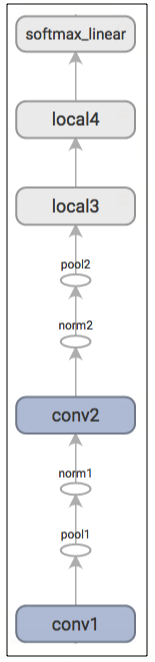
\includegraphics[scale=0.6]{cifar_graph.png}
\end{figure}

练习: inference的输出是未归一化的logits,尝试使用tf.softmax()修改网络架构后返回归一化的预测值。
inputs() 和 inference() 函数提供了评估模型时所需的所有构件,现在我们把将解的重点从构建一个模型转向训练一个模型。

\begin{quote}
练习: inference() 中的模型跟\href{https://code.google.com/p/cuda-convnet/}{cuda-convnet}中描述的CIFAR-10模型有些许不同,其差异主要在于其顶层不是全连接层而是局部连接层,可以尝试修改网络架构来准确的复制全连接模型。
\end{quote}

模型训练
训练一个可进行N维分类的网络的常用方法是使用多项式逻辑回归,又被叫做softmax 回归。Softmax 回归在网络的输出层上附加了一个softmax nonlinearity,并且计算归一化的预测值和label的1-hot encoding的交叉熵。在正则化过程中,我们会对所有学习变量应用权重衰减损失。模型的目标函数是求交叉熵损失和所有权重衰减项的和,loss()函数的返回值就是这个值。
在TensorBoard中使用scalar\_summary来查看该值的变化情况:

\begin{figure}[H]
	\centering
	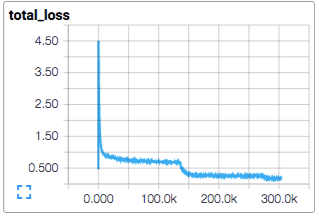
\includegraphics[scale=0.5]{cifar_loss.png}
\end{figure}
我们使用标准的梯度下降算法来训练模型(也可以在Training中看看其他方法),其学习率随时间以指数形式衰减。

\begin{figure}[H]
	\centering
	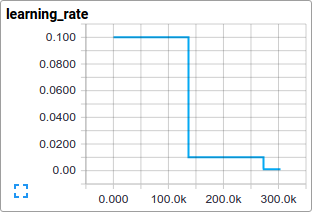
\includegraphics[scale=0.5]{cifar_lr_decay.png}
\end{figure}
\subsection{开始执行并训练模型}
我们已经把模型建立好了,现在通过执行脚本cifar10\_train.py来启动训练过程。
\lstinline[language=Bash]{python cifar10_train.py}
注意: 当第一次在CIFAR-10教程上启动任何任务时,会自动下载CIFAR-10数据集,该数据集大约有160M大小,因此第一次运行时泡杯咖啡小栖一会吧。
你应该可以看到如下类似的输出:
\begin{lstlisting}[language=Python]
Filling queue with 20000 CIFAR images before starting to train. This will take a few minutes.
2015-11-04 11:45:45.927302: step 0, loss = 4.68 (2.0 examples/sec; 64.221 sec/batch)
2015-11-04 11:45:49.133065: step 10, loss = 4.66 (533.8 examples/sec; 0.240 sec/batch)
2015-11-04 11:45:51.397710: step 20, loss = 4.64 (597.4 examples/sec; 0.214 sec/batch)
2015-11-04 11:45:54.446850: step 30, loss = 4.62 (391.0 examples/sec; 0.327 sec/batch)
2015-11-04 11:45:57.152676: step 40, loss = 4.61 (430.2 examples/sec; 0.298 sec/batch)
2015-11-04 11:46:00.437717: step 50, loss = 4.59 (406.4 examples/sec; 0.315 sec/batch)
\end{lstlisting}

脚本会在每10步训练过程后打印出总损失值,以及最后一批数据的处理速度。下面是几点注释:
\begin{itemize}
	\item 第一批数据会非常的慢(大概要几分钟时间),因为预处理线程要把20,000个待处理的CIFAR图像填充到重排队列中;
	\item 打印出来的损失值是最近一批数据的损失值的均值。请记住损失值是交叉熵和权重衰减项的和;
	\item 上面打印结果中关于一批数据的处理速度是在Tesla K40C上统计出来的,如果你运行在CPU上,性能会比此要低;
\end{itemize}

\begin{quote}
练习: 当实验时,第一阶段的训练时间有时会非常的长,长到足以让人生厌。可以尝试减少初始化时初始填充到队列中图片数量来改变这种情况。在cifar10.py中搜索NUM\_EXAMPLES\_PER\_EPOCH\_FOR\_TRAIN并修改之。
\end{quote}

cifar10\_train.py 会周期性的在检查点文件中保存模型中的所有参数,但是不会对模型进行评估。cifar10\_eval.py会使用该检查点文件来测试预测性能(详见下面的描述:评估模型)。
如果按照上面的步骤做下来,你应该已经开始训练一个CIFAR-10模型了。恭喜你!
cifar10\_train.py输出的终端信息中提供了关于模型如何训练的一些信息,但是我们可能希望了解更多关于模型训练时的信息,比如:
\begin{itemize}
	\item 损失是真的在减小还是看到的只是噪声数据?
	\item 为模型提供的图片是否合适?
	\item 梯度、激活、权重的值是否合理?
	\item 当前的学习率是多少?
\end{itemize}

TensorBoard提供了该功能,可以通过cifar10\_train.py中的SummaryWriter周期性的获取并显示这些数据。
比如我们可以在训练过程中查看local3的激活情况,以及其特征维度的稀疏情况:

\begin{figure}[H]
	\centering
	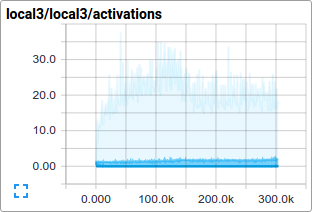
\includegraphics[scale=0.5]{cifar_activations.png}
	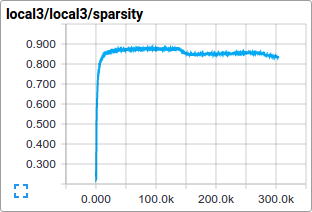
\includegraphics[scale=0.5]{cifar_sparsity.png}
\end{figure}

\subsection{评估模型}
现在可以在另一部分数据集上来评估训练模型的性能。脚本文件cifar10\_eval.py对模型进行了评估,利用 inference()函数重构模型,并使用了在评估数据集所有10,000张CIFAR-10图片进行测试。最终计算出的精度为1:N,N=预测值中置信度最高的一项与图片真实label匹配的频次。(It calculates the precision at 1: how often the top prediction matches the true label of the image)。
为了监控模型在训练过程中的改进情况,评估用的脚本文件会周期性的在最新的检查点文件上运行,这些检查点文件是由cifar10\_train.py产生。
\lstinline[language=Bash]{python cifar10_eval.py}

\begin{quote}
注意:不要在同一块GPU上同时运行训练程序和评估程序,因为可能会导致内存耗尽。尽可能的在其它单独的GPU上运行评估程序,或者在同一块GPU上运行评估程序时先挂起训练程序。
\end{quote}
你可能会看到如下输出

\begin{lstlisting}[language=Bash]
2015-11-06 08:30:44.391206: precision @ 1 = 0.860
...
\end{lstlisting}

评估脚本只是周期性的返回precision@1 (The script merely returns the precision @ 1 periodically)--在该例中返回的准确率是86\%。cifar10\_eval.py 同时也返回其它一些可以在TensorBoard中进行可视化的简要信息。可以通过这些简要信息在评估过程中进一步的了解模型。
训练脚本会为所有学习变量计算其移动均值,评估脚本则直接将所有学习到的模型参数替换成对应的移动均值。这一替代方式可以在评估过程中提升模型的性能。

\begin{quote}
练习: 通过precision @ 1测试发现,使用均值参数可以将预测性能提高约3\%,在cifar10\_eval.py中尝试修改为不采用均值参数的方式,并确认由此带来的预测性能下降。
\end{quote}
\subsection{在多个GPU办卡上训练模型}
现代的工作站可能包含多个GPU进行科学计算。TensorFlow可以利用这一环境在多个GPU卡上运行训练程序。
在并行、分布式的环境中进行训练,需要对训练程序进行协调。对于接下来的描述,术语模型拷贝(model replica)特指在一个数据子集中训练出来的模型的一份拷贝。
如果天真的对模型参数的采用异步方式更新将会导致次优的训练性能,这是因为我们可能会基于一个旧的模型参数的拷贝去训练一个模型。但与此相反采用完全同步更新的方式,其速度将会变得和最慢的模型一样慢(Conversely, employing fully synchronous updates will be as slow as the slowest model replica.)。
在具有多个GPU的工作站中,每个GPU的速度基本接近,并且都含有足够的内存来运行整个CIFAR-10模型。因此我们选择以下方式来设计我们的训练系统:

\begin{itemize}
	\item 在每个GPU上放置单独的模型副本;
	\item 等所有GPU处理完一批数据后再同步更新模型的参数;
\end{itemize}
下图示意了该模型的结构:

\begin{figure}[H]
\centering
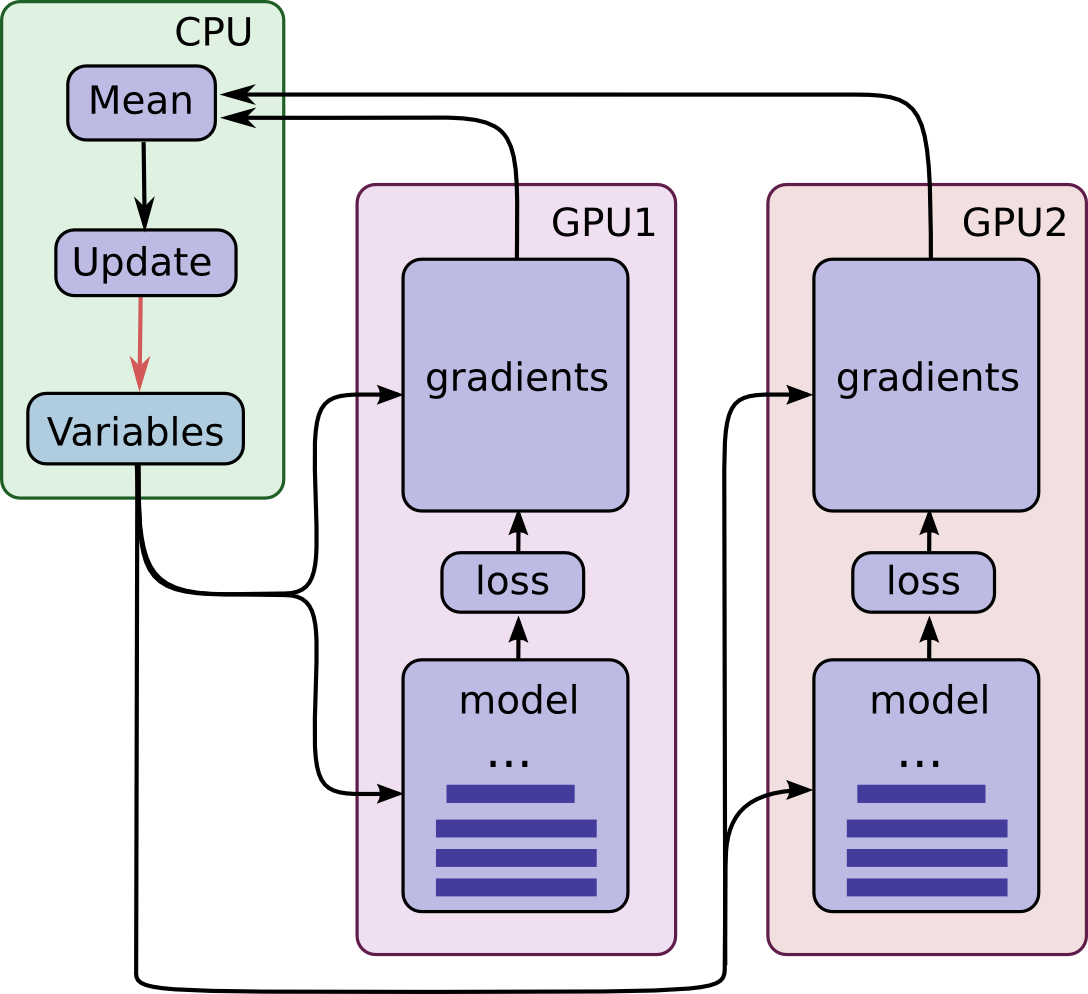
\includegraphics[scale=0.3]{Parallelism.png}
\end{figure}
可以看到,每一个GPU会用一批独立的数据计算梯度和估计值。这种设置可以非常有效的将一大批数据分割到各个GPU上。
这一机制要求所有GPU能够共享模型参数。但是众所周知在GPU之间传输数据非常的慢,因此我们决定在CPU上存储和更新所有模型的参数(对应图中绿色矩形的位置)。这样一来,GPU在处理一批新的数据之前会更新一遍的参数。
图中所有的GPU是同步运行的。所有GPU中的梯度会累积并求平均值(绿色方框部分)。模型参数会利用所有模型副本梯度的均值来更新。
\subsection{在多设备中设置变量和操作}
在多个设备中设置变量和操作时需要做一些特殊的抽象。
我们首先需要把在单个模型拷贝中计算估计值和梯度的行为抽象到一个函数中。在代码中,我们称这个抽象对象为“tower”。对于每一个“tower”我们都需要设置它的两个属性:
在一个tower中为所有操作设定一个唯一的名称。tf.name\_scope()通过添加一个范围前缀来提供该唯一名称。比如,第一个tower中的所有操作都会附带一个前缀tower\_0,示例:tower\_0/conv1/Conv2D;
在一个tower中运行操作的优先硬件设备。 tf.device() 提供该信息。比如,在第一个tower中的所有操作都位于 device('/gpu:0')范围中,暗含的意思是这些操作应该运行在第一块GPU上;
为了在多个GPU上共享变量,所有的变量都绑定在CPU上,并通过tf.get\_variable()访问。可以查看Sharing Variables以了解如何共享变量。

\subsection{启动并在多个GPU上训练模型}
如果你的机器上安装有多块GPU,你可以通过使用cifar10\_multi\_gpu\_train.py脚本来加速模型训练。该脚本是训练脚本的一个变种,使用多个GPU实现模型并行训练。
\lstinline[language=Bash]{python cifar10_multi_gpu_train.py --num_gpus=2}
训练脚本的输出如下所示:

\begin{lstlisting}[language=Bash]
Filling queue with 20000 CIFAR images before starting to train. This will take a few minutes.
2015-11-04 11:45:45.927302: step 0, loss = 4.68 (2.0 examples/sec; 64.221 sec/batch)
2015-11-04 11:45:49.133065: step 10, loss = 4.66 (533.8 examples/sec; 0.240 sec/batch)
2015-11-04 11:45:51.397710: step 20, loss = 4.64 (597.4 examples/sec; 0.214 sec/batch)
2015-11-04 11:45:54.446850: step 30, loss = 4.62 (391.0 examples/sec; 0.327 sec/batch)
2015-11-04 11:45:57.152676: step 40, loss = 4.61 (430.2 examples/sec; 0.298 sec/batch)
2015-11-04 11:46:00.437717: step 50, loss = 4.59 (406.4 examples/sec; 0.315 sec/batch)
...
\end{lstlisting}

需要注意的是默认的GPU使用数是1,此外,如果你的机器上只有一个GPU,那么所有的计算都只会在一个GPU上运行,即便你可能设置的是N个。

\begin{quote}
练习: cifar10\_train.py中的批处理大小默认配置是128。尝试在2个GPU上运行cifar10\_multi\_gpu\_train.py脚本,并且设定批处理大小为64,然后比较2种方式的训练速度
\end{quote}

\subsection{下一步}
恭喜你! 你已经完成了CIFAR-10教程。 如果你对开发和训练自己的图像分类系统感兴趣,我们推荐你新建一个基于该教程的分支,并修改其中的内容以建立解决您问题的图像分类系统。
\begin{quote}
\emph{练习: 下载Street View House Numbers (SVHN) 数据集。新建一个CIFAR-10教程的分支,并将输入数据替换成SVHN。尝试改变网络结构以提高预测性能。}
\end{quote}

\section{RNN}
人不能抓住每一秒的思考,当你读这篇文章的时候,你能基于你之前的对单词的理解明白文章的每一个单词的意思,你思考的时候不需要丢掉所有的东西,你的思想有持续性。\par
传统的神经网络很难做到这点,这也是传统神经网络的主要缺点。例如你想分类电影中的不同时间点的事件,传统神经网络用不清楚如何用之前的事件了解新的事件。\par
RNN通过循环处理这个问题,允许信息保留。\par
\begin{figure}[!ht]
\centering
\includegraphics[scale=0.5]{RNN-rolled.png}
\end{figure}
上面的图表示一个RNN单元,A得到输入$x_t$和输出$h_t$,A允许信息被循环从一步到下一步,一个循环神经网络可以看成是多个相同单元的复制。铺开RNN可以得到
\begin{figure}[!ht]
\centering
\includegraphics[scale=0.3]{RNN-unrolled.png}
\caption{unrolled RNN}
\end{figure}
这个链式结构揭示了循环神经网络和序列或者列表密切相关,它适用于这种数据。
\subsection{The Problem Long-Term Dependencies}
语言模型中常用先前的一个词预测下一个词,如果我们尝试预测"the clouds are in the {\color{red}{sky}}"我们不需要很多上下文信息RNN通过之前的信息就能学到。但是我们尝试预测这样一个句子"I grew up in France... I speak fluent {\color{red}{France}}",之前的信息暗示下一个单词可能是语言的名字,如果我们想去缩小语言的范围,我们需要上下文{\color{red}{France}},可相关信息和这个需要点的间隔很大。
\begin{figure}[!ht]
\centering
\includegraphics[scale=0.3]{RNN-longtermdependencies.png}
\end{figure}
理论上RNN有能力处理“long-term dependencies”,人能小心的挑选参数解决这个烦人的问题,然而不幸的是RNN似乎不能做到,原因由\href{http://www-dsi.ing.unifi.it/~paolo/ps/tnn-94-gradient.pdf}{Hochreiter (1991) [German] and Bengio, et al. (1994)}提出.
\subsection{LSTM网络}
Long Short Term Memory networks通常简称为LSTMs是一个特殊的RNN,能学习learning long-term dependencies,它被\href{http://deeplearning.cs.cmu.edu/pdfs/Hochreiter97_lstm.pdf}{Hochreiter  Schmidhuber (1997)}引入,然后被提炼,在大型文体处理上效果很好因而被广泛的使用。\par
LSTMs明确的设计去解决 long-term dependency problem。\par
所有的循环神经网络都有重复的链式形式。在标准的RNNs,重复的模块有一个非常简单的结构,像tanh Layer。
\begin{figure}
\centering
\includegraphics[scale=0.3]{LSTM3-SimpleRNN.png}
\caption{The repeating module in a standard RNN contains a single layer}
\end{figure}
LSTMs也有这样类似的结构,但是congruent模块有点不同,有一个神经网络层有四个相互作用部分,
\begin{figure}
\centering
\includegraphics[scale=0.3]{LSTM3-chain.png}
\caption{The repeating module in an LSTM contains four interacting layers}
\end{figure}
\begin{figure}
\centering
\includegraphics[scale=0.3]{LSTM2-notation.png}
\end{figure}
在上面的图上,每一根线上携带的都是一个向量,从一个输出节点到其它输入,粉色圆圈代表按点操作,黄色盒子是学习好的神经网络层,线融合表示串联,copy表示将一条线复制一份。
\subsection{LSTMs想法的核心}
LSTMs的核心是图像顶部的水平流过的cell state,cell state像一个传送带,它笔直的沿着整条链跑,和一些次要的线性交互,很容易实现信息不改变的流动。
\begin{figure}
\centering
\includegraphics[scale=0.3]{LSTM3-C-line.png}
\end{figure}
LSTM能删除或者增加信息到cell state,被控制的结构称为门。门是一种让信息通过的手段,由一个sigmoid神经网络层和pointwise惩罚操作组成。
\begin{figure}
\centering
\includegraphics[scale=0.5]{LSTM3-gate.png}
\end{figure}
sigmod Layer输出0到1之间的数,描述多少组件应该被通过,0表示不允许通过1表示让一切通过,LSTMs有三个门,保护和控制cell state。
\subsection{一步步的设置}
第一步是LSTMs决定什么信息应该被传送,这个决定每一个称为忘记门的sigmoid layer组成,通过$h_{t-1}$和$x_t$输出0到1之间的数给当前的$C_{t-1}$,1表示完全保持,0表示丢弃。\par
对于上面的语言模型,cell state也许包含the gender of the present subjects,以至于正确的带名字能被使用,当我们看一个新的subject,我们想图忘记the gender of the old subject。
\begin{figure}
\centering
\includegraphics[scale=0.5]{LSTM3-focus-f.png}
\end{figure}
下一步是决定什么新的信息将被存储在cell state中,这分为两部分
\begin{enumerate}
	\item Sigmod layer调用 input gate layer决定更新哪个值。
	\item tanh layer创建一个可能被添加到state新的候选向量。$\widetilde{C_t}$
\end{enumerate}
下一步我们结合两个不走创建一个更新状态。,在我们的语言模型例子中,我们想要增加gender of the new subject到cell state取代我们将要忘记的数据
\begin{figure}
\centering
\includegraphics[scale=0.5]{LSTM3-focus-i.png}
\end{figure}
现在更新老的cell state$C_{t-1}$到新的cell state$C_t$,我们用老的$c_{t-1}$乘上$f_t$忘记我们之前决定忘记的事,然后我们增加$i_t*\widetilde{C_t}$.这是新的候选值,表示我们更新每个状态值的规模。在例子中的语言模型,我们删掉了一个老的subject's gender增加新的信息。
\begin{figure}
\centering
\includegraphics[scale=0.5]{LSTM3-focus-i.png}
\end{figure}
最后我们需要决定我们输出什么,输出取决于我们的cell state,但是将被过滤,所限我们运行sigmoid layer决定我们将输出那一部分。然后我们放通过tanh将cell state映射到-1,1,然后乘上sigmoid门的输出,以至于我们仅仅输出我们决定输出的部分。\par
对于语言模型的例子,因为它仅仅看subject,它也许想输出关于动词的信息,例子中的下一个,例如,它也许输出是否subject是单数或者复数,以至于从一个动词应该能知道接下来应该是动词的什么形式。
\begin{figure}
\centering
\includegraphics[scale=0.5]{LSTM3-focus-o.png}
\end{figure}
\subsection{LSTM的多种变体}
\href{ftp://ftp.idsia.ch/pub/juergen/TimeCount-IJCNN2000.pdf}{Gers  Schmidhuber (2000)},它增加了peephole connections,这一位置我们让gate layer通过cell state
\begin{figure}
\centering
\includegraphics[scale=0.5]{LSTM3-var-peepholes.png}
\end{figure}
上面的图增加了peepholes到所有的门,但是一些论文给出一些peepholes和not others。另一个变体用两个forget 和输入门。而不是分别决定忘记或者添加信息,我们一起决定,我们需要输入一些值是忘记,我们仅仅忘记老的值输入新值到state
\begin{figure}
\centering
\includegraphics[scale=0.5]{LSTM3-var-tied.png}
\end{figure}
一个更引人注目的变体是Gate Recurrent Unit或者称为(GRU),由\href{http://arxiv.org/pdf/1406.1078v3.pdf}{Cho, et al. (2014)}引入,它结合忘记和输入门为一个单独的更新们,它也融合cell state和hidden state做了些改变,这结果模型比标准的LSTM模型简单,现在也越来越流行。
\begin{figure}
\centering
\includegraphics[scale=0.5]{LSTM3-var-GRU.png}
\end{figure}
这些仅仅是非常流行的LSTM变体,有一些其它的像\href{http://arxiv.org/pdf/1508.03790v2.pdf}{Yao, et al. (2015)}的Depth Gated RNNs,用完全不同的方法处理long-term dependencies,像\href{http://arxiv.org/pdf/1402.3511v1.pdf}{Koutnik, et al. (2014)}的Clockwork RNNs。\par
那个算法是最好的?它们的差别大吗?\href{http://arxiv.org/pdf/1503.04069.pdf}{Greff, et al. (2015) }做了一些比较了一些流行的变体,发现它们基本相同。
\href{http://jmlr.org/proceedings/papers/v37/jozefowicz15.pdf}{Jozefowicz, et al. (2015)}比较了超过1万中架构,找到了一些在确定问题上比LSTMs好的架构。
\section{向量字表示}
\subsection{Vector Representation of Words}
通常图像或音频系统处理的是由图片中所有单个原始像素点强度值或者音频中功率谱密度的强度值,把它们编码成丰富、高维度的向量数据集。对于物体或语音识别这一类的任务,我们所需的全部信息已经都存储在原始数据中(显然人类本身就是依赖原始数据进行日常的物体或语音识别的)。然后,自然语言处理系统通常将词汇作为离散的单一符号,例如 "cat" 一词或可表示为 Id537 ,而 "dog" 一词或可表示为 Id143。这些符号编码毫无规律,无法提供不同词汇之间可能存在的关联信息。换句话说,在处理关于 "dogs" 一词的信息时,模型将无法利用已知的关于 "cats" 的信息(例如,它们都是动物,有四条腿,可作为宠物等等)。可见,将词汇表达为上述的独立离散符号将进一步导致数据稀疏,使我们在训练统计模型时不得不寻求更多的数据。而词汇的向量表示将克服上述的难题。向量空间模型 (VSMs)将词汇表达(嵌套)于一个连续的向量空间中,语义近似的词汇被映射为相邻的数据点。向量空间模型在自然语言处理领域中有着漫长且丰富的历史,不过几乎所有利用这一模型的方法都依赖于 分布式假设,其核心思想为出现于上下文情景中的词汇都有相类似的语义。采用这一假设的研究方法大致分为以下两类:基于计数的方法 (e.g. 潜在语义分析), 和 预测方法 (e.g. 神经概率化语言模型).

其中它们的区别在如下论文中又详细阐述 \href{http://clic.cimec.unitn.it/marco/publications/acl2014/baroni-etal-countpredict-acl2014.pdf}{Baroni :et al},不过简而言之:基于计数的方法计算某词汇与其邻近词汇在一个大型语料库中共同出现的频率及其它统计量,然后将这些统计量映射到一个小型且稠密的向量中。预测方法则试图直接从某词汇的邻近词汇对其进行预测,在此过程中利用已经学习到的小型且稠密的嵌套向量。

Word2vec是一种可以进行高效率词嵌套学习的预测模型。其两种变体分别为:连续词袋模型(CBOW)及Skip-Gram模型。从算法角度看,这两种方法非常相似,其区别为CBOW根据源词上下文词汇('the cat sits on the')来预测目标词汇(例如,‘mat’),而Skip-Gram模型做法相反,它通过目标词汇来预测源词汇。Skip-Gram模型采取CBOW的逆过程的动机在于:CBOW算法对于很多分布式信息进行了平滑处理(例如将一整段上下文信息视为一个单一观察量)。很多情况下,对于小型的数据集,这一处理是有帮助的。相形之下,Skip-Gram模型将每个“上下文-目标词汇”的组合视为一个新观察量,这种做法在大型数据集中会更为有效。本教程余下部分将着重将解Skip-Gram模型。
\subsection{处理噪声的对比训练}
神经概率化语言模型通常使用极大似然法 (ML) 进行训练,其中通过 softmax function 来最大化当提供前一个单词 h (代表 "history"),后一个单词的概率$w_t$(目标词概率)
\begin{equation*}
P(w_t|h)=softmax(score(w_t,h))=\frac{exp\left\{score(w_t,h)\right\}}{\Sigma_{Word w' in Vocab}exp\left\{score(w',h)\right\}}
\end{equation*}
当 $score(w_t,h)$ 计算了文字 $w_t$ 和 上下文 h 的相容性(通常使用向量积)。我们使用对数似然函数来训练训练集的最大值,比如通过:
\begin{equation*}
J_{ML} = logP(w_t|h)=score(w_t,h)-log(\Sigma_{Word w' in Vocab}exp\left\{score(w',h)\right\})
\end{equation*}
这里提出了一个解决语言概率模型的合适的通用方法。然而这个方法实际执行起来开销非常大,因为我们需要去计算并正则化当前上下文环境 h 中所有其它 V 单词 w' 的概率得分,在每一步训练迭代中。
\begin{figure}[H]
\includegraphics[scale=0.5]{softmax-nplm.png}
\caption{CBOW方法}
\end{figure}
从另一个角度来说,当使用word2vec模型时,我们并不需要对概率模型中的所有特征进行学习。而CBOW模型和Skip-Gram模型为了避免这种情况发生,使用一个二分类器(逻辑回归)在同一个上下文环境里从 k 虚构的 (噪声) 单词$\hat{w}$区分真正的目标单词$w_t$,下面详细参数CBOW模型,对于Skip-Gram模型只要简单的反向操作即可。
\begin{center}
\begin{figure}[H]
\includegraphics[scale=0.5]{nce-nplm.png}
\caption{Skip-Gram}
\end{figure}
\end{center}
从数学的角度来说,我们的目标是对每个样本最大化:
\begin{equation*}
J_{NEG}=logQ_{\theta}(D=1|w_t,h)+k\underset{\hat{w}\sim P_{noise}}{E}[logQ_{\theta}(D=0|\hat{\omega},h)]
\end{equation*}
其中$Q_{\theta}(D=1|w,h)$代表的是当前上下文h,根据所学得嵌套向量$\theta$目标单词 w 使用二分类逻辑回归计算得出的概率。在实践中,我们通过在噪声分布中绘制比对文字来获得近似的期望值(通过计算\href{https://en.wikipedia.org/wiki/Monte_Carlo_integration}{蒙特卡洛平均值})。

当真实地目标单词被分配到较高的概率,同时噪声单词的概率很低时,目标函数也就达到最大值了。从技术层面来说,这种方法叫做\href{http://papers.nips.cc/paper/5021-distributed-representations-of-words-and-phrases-and-their-compositionality.pdf}{负抽样},而且使用这个损失函数在数学层面上也有很好的解释:这个更新过程也近似于softmax函数的更新。这在计算上将会有很大的优势,因为当计算这个损失函数时,只是有我们挑选出来的 k 个 噪声单词,而没有使用整个语料库 V。这使得训练变得非常快。我们实际上使用了与\href{http://papers.nips.cc/paper/5165-learning-word-embeddings-efficiently-with-noise-contrastive-estimation.pdf}{noise-contrastive estimation (NCE)}介绍的非常相似的方法,这在TensorFlow中已经封装了一个很便捷的函数tf.nn.nce\_loss()。

\subsection{Skip-gram模型}
下面来看一下这个数据集

the quick brown fox jumped over the lazy dog

我们首先对一些单词以及它们的上下文环境建立一个数据集。我们可以以任何合理的方式定义‘上下文’,而通常上这个方式是根据文字的句法语境的(使用语法原理的方式处理当前目标单词可以看一下这篇文献 \href{https://levyomer.files.wordpress.com/2014/04/dependency-based-word-embeddings-acl-2014.pdf}{Levy et al.},比如说把目标单词左边的内容当做一个‘上下文’,或者以目标单词右边的内容,等等。现在我们把目标单词的左右单词视作一个上下文, 使用大小为1的窗口,这样就得到这样一个由(上下文, 目标单词) 组成的数据集:

([the, brown], quick), ([quick, fox], brown), ([brown, jumped], fox), ...

前文提到Skip-Gram模型是把目标单词和上下文颠倒过来,所以在这个问题中,举个例子,就是用'quick'来预测 'the' 和 'brown' ,用 'brown' 预测 'quick' 和 'fox' 。因此这个数据集就变成由(输入, 输出)组成的:

(quick, the), (quick, brown), (brown, quick), (brown, fox), ...

目标函数通常是对整个数据集建立的,但是本问题中要对每一个样本(或者是一个batch\_size 很小的样本集,通常设置为16 <= batch\_size <= 512)在同一时间执行特别的操作,称之为\href{https://en.wikipedia.org/wiki/Stochastic_gradient_descent}{随机梯度下降 (SGD)}。我们来看一下训练过程中每一步的执行。

假设用 t 表示上面这个例子中quick 来预测 the 的训练的单个循环。用 num\_noise 定义从噪声分布中挑选出来的噪声(相反的)单词的个数,通常使用一元分布,P(w)。为了简单起见,我们就定num\_noise=1,用 sheep 选作噪声词。接下来就可以计算每一对观察值和噪声值的损失函数了,每一个执行步骤就可表示为:
\begin{equation*}
J_{NEG}^{(t)}=logQ_{\theta}(D=1|the,quick)+log(Q_{\theta}(D=0|sleep,quick))
\end{equation*}
整个计算过程的目标是通过更新嵌套参数$\theta$来逼近目标函数(这个例子中就是使目标函数最大化)。为此我们要计算损失函数中嵌套参数$\theta$的梯度,比如\[\frac{\partial}{\partial}J_{NEG}\]
(幸好TensorFlow封装了工具函数可以简单调用!)。对于整个数据集,当梯度下降的过程中不断地更新参数,对应产生的效果就是不断地移动每个单词的嵌套向量,直到可以把真实单词和噪声单词很好得区分开。

我们可以把学习向量映射到2维中以便我们观察,其中用到的技术可以参考 \href{http://lvdmaaten.github.io/tsne/}{t-SNE 降维技术}。当我们用可视化的方式来观察这些向量,就可以很明显的获取单词之间语义信息的关系,这实际上是非常有用的。当我们第一次发现这样的诱导向量空间中,展示了一些特定的语义关系,这是非常有趣的,比如文字中 male-female,gender 甚至还有 country-capital 的关系, 如下方的图所示 (也可以参考 \href{http://www.aclweb.org/anthology/N13-1090}{Mikolov et al.}, 2013论文中的例子)。
\begin{center}
\begin{figure}[H]
\includegraphics[scale=0.5]{linear-relationships.png}
\end{figure}
\end{center}
这也解释了为什么这些向量在传统的NLP问题中可作为特性使用,比如用在对一个演将章节打个标签,或者对一个专有名词的识别 (看看如下这个例子 \href{https://arxiv.org/pdf/1103.0398v1.pdf}{Collobert et al.}或者 \href{http://www.aclweb.org/anthology/P10-1040}{Turian et al.})。

不过现在让我们用它们来画漂亮的图表吧!

这里谈得都是嵌套,那么先来定义一个嵌套参数矩阵。我们用唯一的随机值来初始化这个大矩阵。
\begin{lstlisting}[language=Python]
embeddings = tf.Variable(
    tf.random_uniform([vocabulary_size, embedding_size], -1.0, 1.0))
\end{lstlisting}
对噪声-比对的损失计算就使用一个逻辑回归模型。对此,我们需要对语料库中的每个单词定义一个权重值和偏差值。(也可称之为输出权重 与之对应的 输入嵌套值)。定义如下:
\begin{lstlisting}[language=Python]
nce_weights = tf.Variable(
  tf.truncated_normal([vocabulary_size, embedding_size],
                      stddev=1.0 / math.sqrt(embedding_size)))
nce_biases = tf.Variable(tf.zeros([vocabulary_size]))
\end{lstlisting}我们有了这些参数之后,就可以定义Skip-Gram模型了。简单起见,假设我们已经把语料库中的文字整型化了,这样每个整型代表一个单词(细节请查看\_basic.py)。Skip-Gram模型有两个输入。一个是一组用整型表示的上下文单词,另一个是目标单词。给这些输入建立占位符节点,之后就可以填入数据了。
\begin{lstlisting}[language=Python]
train_inputs = tf.placeholder(tf.int32, shape=[batch_size])
train_labels = tf.placeholder(tf.int32, shape=[batch_size, 1])
\end{lstlisting}
然后我们需要对批数据中的单词建立嵌套向量,TensorFlow提供了方便的工具函数。
\begin{lstlisting}[language=Python]
embed = tf.nn.embedding_lookup(embeddings, train_inputs)
\end{lstlisting}
好了,现在我们有了每个单词的嵌套向量,接下来就是使用噪声-比对的训练方式来预测目标单词。
\begin{lstlisting}[language=Python]
loss = tf.reduce_mean(
  tf.nn.nce_loss(nce_weights, nce_biases, embed, train_labels,
                 num_sampled, vocabulary_size))
\end{lstlisting}
我们对损失函数建立了图形节点,然后我们需要计算相应梯度和更新参数的节点,比如说在这里我们会使用随机梯度下降法,TensorFlow也已经封装好了该过程。
\begin{lstlisting}[language=Python]
optimizer = tf.train.GradientDescentOptimizer(learning_rate=1.0).minimize(loss)
\end{lstlisting}
\subsection{训练过程}
训练的过程很简单,只要在循环中使用feed\_dict不断给占位符填充数据,同时调用 session.run即可。
\begin{lstlisting}[language=Python]
for inputs, labels in generate_batch(...):
  feed_dict = {training_inputs: inputs, training_labels: labels}
  _, cur_loss = session.run([optimizer, loss], feed_dict=feed_dict)
\end{lstlisting}
\subsection{嵌套学习结果可视化}
\begin{center}
\begin{figure}[H]
\includegraphics[scale=0.5]{tsne.png}
\end{figure}
\end{center}
Et voila! 与预期的一样,相似的单词被聚类在一起。对word2vec模型更复杂的实现需要用到TensorFlow一些更高级的特性,具体是实现可以参考\href{https://github.com/bleedingfight/models/tree/master/tutorials/embedding}{word2vec.py}
\subsection{嵌套学习的评估:类比推理}
词嵌套在NLP的预测问题中是非常有用且使用广泛地。如果要检测一个模型是否是可以成熟地区分词性或者区分专有名词的模型,最简单的办法就是直接检验它的预测词性、语义关系的能力,比如让它解决形如king is to queen as father is to ?这样的问题。这种方法叫做类比推理 ,可参考Mikolov and colleagues,数据集下载地址为:\href{https://word2vec.googlecode.com/svn/trunk/questions-words.txt}{questions-words.txt} 。
To see how we do this evaluation如何执行这样的评估,可以看build\_eval\_graph()和 eval()这两个函数在下面源码中的使用 \href{https://github.com/bleedingfight/models/tree/master/tutorials/embedding}{word2vec.py}

超参数的选择对该问题解决的准确性有巨大的影响。想要模型具有很好的表现,需要有一个巨大的训练数据集,同时仔细调整参数的选择并且使用例如二次抽样的一些技巧。不过这些问题已经超出了本教程的范围。
\subsection{优化实现}
以上简单的例子展示了TensorFlow的灵活性。比如说,我们可以很轻松得用现成的tf.nn.sampled\_softmax\_loss()来代替tf.nn.nce\_loss()构成目标函数。如果你对损失函数想做新的尝试,你可以用TensorFlow手动编写新的目标函数的表达式,然后用控制器执行计算。这种灵活性的价值体现在,当我们探索一个机器学习模型时,我们可以很快地遍历这些尝试,从中选出最优。

一旦你有了一个满意的模型结构,或许它就可以使实现运行地更高效(在短时间内覆盖更多的数据)。比如说,在本教程中使用的简单代码,实际运行速度都不错,因为我们使用Python来读取和填装数据,而这些在TensorFlow后台只需执行非常少的工作。如果你发现你的模型在输入数据时存在严重的瓶颈,你可以根据自己的实际问题自行实现一个数据阅读器,参考 新的数据格式。对于Skip-Gram 模型,我们已经完成了如下这个例子 \href{https://github.com/bleedingfight/models/tree/master/tutorials/embedding}{word2vec.py}。

如果I/O问题对你的模型已经不再是个问题,并且想进一步地优化性能,或许你可以自行编写TensorFlow操作单元,详见 添加一个新的操作。相应的,我们也提供了Skip-Gram模型的例子 \href{https://github.com/bleedingfight/models/tree/master/tutorials/embedding}{optimized.py}。请自行调节以上几个过程的标准,使模型在每个运行阶段有更好地性能。
\subsection{RNN}
此教程将展示如何在高难度的语言模型中训练循环神经网络。该问题的目标是获得一个能确定语句概率的概率模型。为了做到这一点,通过之前已经给出的词语来预测后面的词语。我们将使用 PTB(Penn Tree Bank) 数据集,这是一种常用来衡量模型的基准,同时它比较小而且训练起来相对快速。

语言模型是很多有趣难题的关键所在,比如语音识别,机器翻译,图像字幕等。它很有意思--可以参看 here。

本教程的目的是重现 \href{http://arxiv.org/abs/1409.2329}{Zaremba et al., 2014} 的成果,它们在 PTB 数据集上得到了很棒的结果。
\subsection{下载及准备数据}
本教程需要的数据在 data/ 路径下,来源于 Tomas Mikolov 网站上的\href{http://www.fit.vutbr.cz/~imikolov/rnnlm/simple-examples.tg}{PTB 数据集}

该数据集已经预先处理过并且包含了全部的 10000 个不同的词语,其中包括语句结束标记符,以及标记稀有词语的特殊符号 (<unk>) 。我们在 reader.py 中转换所有的词语,让它们各自有唯一的整型标识符,便于神经网络处理。
\subsection{LSTM}
模型的核心由一个 LSTM 单元组成,其可以在某时刻处理一个词语,以及计算语句可能的延续性的概率。网络的存储状态由一个零矢量初始化并在读取每一个词语后更新。而且,由于计算上的原因,我们将以 batch\_size 为最小批量来处理数据。

基础的伪代码就像下面这样:
\begin{lstlisting}[language=Python]
lstm = rnn_cell.BasicLSTMCell(lstm_size)
state = tf.zeros([batch_size, lstm.state_size])

loss = 0.0
for current_batch_of_words in words_in_dataset:
    output, state = lstm(current_batch_of_words, state)

    logits = tf.matmul(output, softmax_w) + softmax_b
    probabilities = tf.nn.softmax(logits)
    loss += loss_function(probabilities, target_words)
\end{lstlisting}
\subsection{截断反向传播}
为使学习过程易于处理,通常的做法是将反向传播的梯度在(按时间)展开的步骤上照一个固定长度(num\_steps)截断。 通过在一次迭代中的每个时刻上提供长度为 num\_steps 的输入和每次迭代完成之后反向传导,这会很容易实现。

一个简化版的用于计算图创建的截断反向传播代码:
\begin{lstlisting}[language=Python]
words = tf.placeholder(tf.int32, [batch_size, num_steps])

lstm = rnn_cell.BasicLSTMCell(lstm_size)
initial_state = state = tf.zeros([batch_size, lstm.state_size])

for i in range(len(num_steps)):
    output, state = lstm(words[:, i], state)

    # ...

final_state = state
\end{lstlisting}
下面展现如何实现迭代整个数据集:
\begin{lstlisting}[language=Python]
numpy_state = initial_state.eval()
total_loss = 0.0
for current_batch_of_words in words_in_dataset:
    numpy_state, current_loss = session.run([final_state, loss],
        feed_dict={initial_state: numpy_state, words: current_batch_of_words})
    total_loss += current_loss
\end{lstlisting}
\subsection{输入}
在输入 LSTM 前,词语 ID 被嵌入到了一个密集的表示中(查看 矢量表示教程)。这种方式允许模型高效地表示词语,也便于写代码:
\begin{lstlisting}[language=Python]
# embedding_matrix 张量的形状是: [vocabulary_size, embedding_size]
word_embeddings = tf.nn.embedding_lookup(embedding_matrix, word_ids)
\end{lstlisting}
嵌入的矩阵会被随机地初始化,模型会学会通过数据分辨不同词语的意思。
\subsection{损失函数}
我们想使目标词语的平均负对数概率最小$loss = -\frac{1}{N}\Sigma_{i=1}^NlnP_{target_i}$
实现起来并非很难,而且函数 sequence\_loss\_by\_example 已经有了,可以直接使用。

论文中的典型衡量标准是每个词语的平均困惑度(perplexity),计算式为
$$e^{-\frac{1}{N}\Sigma_{i=1}^N}lnp_{target_i}=e^{loss}$$
同时我们会观察训练过程中的困惑度值(perplexity)
\subsection{多个LSTM层堆叠}
要想给模型更强的表达能力,可以添加多层 LSTM 来处理数据。第一层的输出作为第二层的输入,以此类推。

类 MultiRNNCell 可以无缝的将其实现:
\begin{lstlisting}[language=Python]
lstm = rnn_cell.BasicLSTMCell(lstm_size)
stacked_lstm = rnn_cell.MultiRNNCell([lstm] * number_of_layers)

initial_state = state = stacked_lstm.zero_state(batch_size, tf.float32)
for i in range(len(num_steps)):
    # 每次处理一批词语后更新状态值.
    output, state = stacked_lstm(words[:, i], state)

    # 其余的代码.
    # ...

final_state = state
\end{lstlisting}
\subsection{编译并运行代码}
首先需要构建库,在CPU上编译:
\begin{lstlisting}[language=Python]
bazel build -c opt tensorflow/models/rnn/ptb:ptb_word_lm
\end{lstlisting}
如果你有一个强大的 GPU,可以运行
\begin{lstlisting}[language=Python]
bazel build -c opt --config=cuda tensorflow/models/rnn/ptb:ptb_word_lm
\end{lstlisting}
运行模型:
\begin{lstlisting}[language=Python]
bazel-bin/tensorflow/models/rnn/ptb/ptb_word_lm \
  --data_path=/tmp/simple-examples/data/ --alsologtostderr --model small
\end{lstlisting}
教程代码中有 3 个支持的模型配置参数:"small", "medium" 和 "large"。它们指的是 LSTM 的大小,以及用于训练的超参数集。

模型越大,得到的结果应该更好。在测试集中 small 模型应该可以达到低于 120 的困惑度(perplexity),large 模型则是低于 80,但它可能花费数小时来训练。

\section{图像识别}
我们的大脑看东西很简单,它不需要得到任何人的告诉就能分别狮子,鲸钱包,读一个符号或者识别人脸,
但是计算机解决这个问题却很难。最近几年机器学习已经在这个问题上取得了很大的进步,事实上我们已经发现了一个称谓CNN的模型可以在很难的视觉认知邻域上获得匹敌甚至超过人类的性能。研究人员在ImageNet上展示它们的计算机视觉的成果,模型性能持续提升从\href{http://static.googleusercontent.com/media/research.google.com/en//archive/unsupervised_icml2012.pdf}{QuocNet},\href{http://www.cs.toronto.edu/~fritz/absps/imagenet.pdf}{AlexNet},\href{http://arxiv.org/abs/1409.4842}{Inception(GoogleNet)},\href{http://arxiv.org/abs/1502.03167}{BN-inception-v2},Google累不和外部的研究人员都已经出版了一些论文描述这些模型,但是结果任然河南再次提升,我们用下面的代码实现我们最新的模型\href{http://arxiv.org/abs/1512.00567}{Inception-v3},Inception-v3 2012年在Imagenet的LVRC上训练,这对计算机来说是一个基本的任务,这里模型尝试着分类整个图形为1000中分类像"斑马","大麦町犬","洗碗机",下面是AlexNet分类的一些图像:
\begin{center}
\begin{figure}[H]
	\centering
	\includegraphics[scale=0.3]{AlexClassification.png}
\end{figure}
\end{center}
为了对比模型,我们检查迷行预测正确结果为"top-5 error rate",AlexNet2012年的验证数据集上得到top-5 error rate 15.3\%,Inception(GoogleLeNet)得到6.67\%,BN-Inception-v2得到4.9\%,Inception-v3得到3.46\%。
\begin{quote}
\emph{人类在ImageNet中做的怎么样,由 Andrej Karpathy 的\href{http://karpathy.github.io/2014/09/02/what-i-learned-from-competing-against-a-convnet-on-imagenet/}{博客}尝试测量人们的性能,它得到了5.1\%的top-5 error rate}
\end{quote}
下面的导航将教你如何使用Inception-v3.你将学习用Python或者C++学习分类图像成1000类,我们也将讨论如何从模型提取高级特征重用到其它的视觉任务。
\subsection{用Python API}
第一次运行时classify\_image.py将从tensorflow官网下载训练好的模型,你将需要200M左右的硬盘空间。开始从github上clone\href{https://github.com/tensorflow/models}{Google模型},然后运行命令:
\begin{lstlisting}[language=Python][language=Bash]
cd models/tutorials/image/imagenet
python classify_image.py
\end{lstlisting}
上面的命令将分类下面的熊猫图片。
\begin{center}
\begin{figure}[H]
\centering
\includegraphics{cropped_panda.jpg}
\end{figure}
\end{center}
如果模型正确运行将生成下面的输出:
\begin{lstlisting}[language=Python]{language=Python}
giant panda, panda, panda bear, coon bear, Ailuropoda melanoleuca (score = 0.88493)
indri, indris, Indri indri, Indri brevicaudatus (score = 0.00878)
lesser panda, red panda, panda, bear cat, cat bear, Ailurus fulgens (score = 0.00317)
custard apple (score = 0.00149)
earthstar (score = 0.00127)
\end{lstlisting}
如果你希望添加其它的JPEG图片,你也许需要编辑--image\_file参数,如果你需要下载模型数据到不同的目录,你将需要指定--model\_dir到使用的目录。
\subsection{用C++ API}
你可以在生产环境上使用C++运行相同的Inception-v3模型。你可以下载包含像这样定义的GraphDef的打包文件
(从TensorFlow仓库的根目录运行)
\begin{lstlisting}[language=Python][language=Bash]
curl -L "https://storage.googleapis.com/download.tensorflow.org/models/inception_v3_2016_08_28_frozen.pb.tar.gz" |
  tar -C tensorflow/examples/label_image/data -xz
\end{lstlisting}
下一步我们编译包含C++代码载入的二进制运行图,如果你已经按照\href{https://www.tensorflow.org/install/install_sources}{the instructions to download the source installation of TensorFlow}
配置了你的平台,你将能在shell终端通过下面的命令构建例子运行:
\begin{lstlisting}[language=Python][language=Bash]
bazel build tensorflow/examples/label_image/...
\end{lstlisting}
你可以像这样创建一个二进制的执行文件:
\begin{lstlisting}[language=Python][language=Bash]
bazel-bin/tensorflow/examples/label_image/label_image
\end{lstlisting}
用框架默认的例子图片,输出下面的结果:
\begin{lstlisting}[language=Python][language=Bash]
I tensorflow/examples/label_image/main.cc:206] military uniform (653): 0.834306
I tensorflow/examples/label_image/main.cc:206] mortarboard (668): 0.0218692
I tensorflow/examples/label_image/main.cc:206] academic gown (401): 0.0103579
I tensorflow/examples/label_image/main.cc:206] pickelhaube (716): 0.00800814
I tensorflow/examples/label_image/main.cc:206] bulletproof vest (466): 0.00535088
\end{lstlisting}
在这个例子中你用一张默认的图片\href{https://en.wikipedia.org/wiki/Grace_Hopper}{Admiral Grace Hopper},你可以看到网络正确识别她的军官制服,得分0.8。
\begin{center}
\begin{figure}[H]
\centering
\includegraphics{grace_hopper.jpg}
\end{figure}
\end{center}
下一步提供--image=参数分辨你的图片
\begin{lstlisting}[language=Python][language=Bash]
bazel-bin/tensorflow/examples/label_image/label_image --image=my_image.png
\end{lstlisting}
如果你查看\href{https://github.com/tensorflow/tensorflow/blob/master/tensorflow/examples/label_image/main.cc}{tensorflow/examples/label\_image/main.cc}你可以明白它是如何工作的,我们希望代码能帮你整合TensorFlow到你的应用,因此我们将一步步的浏览主函数。命令行参数控制文件从哪里载入,即输入图像的内容。模型希望得到$299\times299$的RGB图像,分别是input\_width,input\_height,我们需要缩放图像的像素从0-255到图能操作的一个浮点值。我们通过input\_mean和input\_std控制缩放:我们首先用像素值减去input\_mean然后除以input\_std,这些值看起来可能有点琢磨不透,但是它们被原始作者定义,她/它想训练的时候什么值被匹配,你可以看看我们如何在\href{https://github.com/tensorflow/tensorflow/blob/master/tensorflow/examples/label_image/main.cc#L88}{ReadTensorFromImageFile()}函数中如何应用一张图像。
\begin{lstlisting}[language=Python][language=C++]
// Given an image file name, read in the data, try to decode it as an image,
// resize it to the requested size, and then scale the values as desired.
Status ReadTensorFromImageFile(string file_name, const int input_height,
                               const int input_width, const float input_mean,
                               const float input_std,
                               std::vector<Tensor>* out_tensors) {
  tensorflow::GraphDefBuilder b;
\end{lstlisting}
我们开始创建一个GraphDefBuilder对象指定一个运行或者载入的模型。
\begin{lstlisting}[language=Python][language=C++]
  string input_name = "file_reader";
  string output_name = "normalized";
  tensorflow::Node* file_reader =
      tensorflow::ops::ReadFile(tensorflow::ops::Const(file_name, b.opts()),
                                b.opts().WithName(input_name));
\end{lstlisting}
然后我们开始为我们想要运行或者载入的小模型创建节点,变换大小,缩放像素值得到主函数希望得到的结果,我们创建的第一个节点是保持图像名字的tensor想要载入Const操作然后作为第一个输入传入ReadFile操作,你也许注意到我们传递b.opts()操作给所有的创建操作,参数确保节点被添加到GraphDefBuilder的模型定义。这给了一个名字给节点,
对于给一个名字节点不是严格需要的因为如果你不指定这个将自动命名,但是它使得调试变得简单
\begin{lstlisting}[language=Python][language=C++]
  // Now try to figure out what kind of file it is and decode it.
  const int wanted_channels = 3;
  tensorflow::Node* image_reader;
  if (tensorflow::StringPiece(file_name).ends_with(".png")) {
    image_reader = tensorflow::ops::DecodePng(
        file_reader,
        b.opts().WithAttr("channels", wanted_channels).WithName("png_reader"));
  } else {
    // Assume if it's not a PNG then it must be a JPEG.
    image_reader = tensorflow::ops::DecodeJpeg(
        file_reader,
        b.opts().WithAttr("channels", wanted_channels).WithName("jpeg_reader"));
  }
  // Now cast the image data to float so we can do normal math on it.
  tensorflow::Node* float_caster = tensorflow::ops::Cast(
      image_reader, tensorflow::DT_FLOAT, b.opts().WithName("float_caster"));
  // The convention for image ops in TensorFlow is that all images are expected
  // to be in batches, so that they're four-dimensional arrays with indices of
  // [batch, height, width, channel]. Because we only have a single image, we
  // have to add a batch dimension of 1 to the start with ExpandDims().
  tensorflow::Node* dims_expander = tensorflow::ops::ExpandDims(
      float_caster, tensorflow::ops::Const(0, b.opts()), b.opts());
  // Bilinearly resize the image to fit the required dimensions.
  tensorflow::Node* resized = tensorflow::ops::ResizeBilinear(
      dims_expander, tensorflow::ops::Const({input_height, input_width},
                                            b.opts().WithName("size")),
      b.opts());
  // Subtract the mean and divide by the scale.
  tensorflow::ops::Div(
      tensorflow::ops::Sub(
          resized, tensorflow::ops::Const({input_mean}, b.opts()), b.opts()),
      tensorflow::ops::Const({input_std}, b.opts()),
      b.opts().WithName(output_name));
\end{lstlisting}
我们然后添加更多的节点解码文件数据为图片,转化整数为浮点值,变形然后最后运行减去和除法操作:
\begin{lstlisting}[language=Python][language=C++]
  // This runs the GraphDef network definition that we've just constructed, and
  // returns the results in the output tensor.
  tensorflow::GraphDef graph;
  TF_RETURN_IF_ERROR(b.ToGraphDef(&graph));
\end{lstlisting}
在这最后我们有一个存储在变量b中的模型定义我们用ToGraphDef()转化完整的图定义
\begin{lstlisting}[language=Python][language=C++]
  std::unique_ptr<tensorflow::Session> session(
      tensorflow::NewSession(tensorflow::SessionOptions()));
  TF_RETURN_IF_ERROR(session->Create(graph));
  TF_RETURN_IF_ERROR(session->Run({}, {output_name}, {}, out_tensors));
  return Status::OK();
\end{lstlisting}
我们创建一个运行图的接口tf.Session对象,运行它,指定我们想从那个节点获得输出和放输出数据到哪里,这给我们一个Tensor对象的向量,这个对象将变成一个三个对量,你可以将Tensor认为是多维数组,它保存299像素宽,299像素高。3通道的图像作为浮点值,如果你有自己的图像处理框架,你应该能用它替代,只要你在输入图像到主图中时应用相同的转换。这是用C++创建一个简单的TensorFlow图的例子,但是对于预先训练好的Inception模型我们想从文件载入一个大的定义,你可以在LoadGraph()函数中查看我们如何做的:
\begin{lstlisting}[language=Python][language=C++]
// Reads a model graph definition from disk, and creates a session object you
// can use to run it.
Status LoadGraph(string graph_file_name,
                 std::unique_ptr<tensorflow::Session>* session) {
  tensorflow::GraphDef graph_def;
  Status load_graph_status =
      ReadBinaryProto(tensorflow::Env::Default(), graph_file_name, &graph_def);
  if (!load_graph_status.ok()) {
    return tensorflow::errors::NotFound("Failed to load compute graph at '",
                                        graph_file_name, "'");
  }
\end{lstlisting}
如果你已经查看的图像载入代码,一些名词应该很熟悉。想必须用一个GraphDefBuffer残生一个GraphDef对象,我们载入一个包含GraphDef的protobuf文件。
\begin{lstlisting}[language=Python][language=C++]
  session->reset(tensorflow::NewSession(tensorflow::SessionOptions()));
  Status session_create_status = (*session)->Create(graph_def);
  if (!session_create_status.ok()) {
    return session_create_status;
  }
  return Status::OK();
}
\end{lstlisting}
我们从GraphDef创建一个Session对象传递它给调用器以至于我们稍后能使用。GetTopLabels()函数有些像函数载入,但是我们希望运行主图得到结果,存储它进一个按照标签最高评分的结果,像图片载入,它创建一个的GraphDefBuilder,添加一对节点上去然后运行短图割刀一对输出tensor,在这个例子中它们代表排序的分数和最好可能性的结果的索引位置。
\begin{lstlisting}[language=Python][language=C++]
// Analyzes the output of the Inception graph to retrieve the highest scores and
// their positions in the tensor, which correspond to categories.
Status GetTopLabels(const std::vector<Tensor>& outputs, int how_many_labels,
                    Tensor* indices, Tensor* scores) {
  tensorflow::GraphDefBuilder b;
  string output_name = "top_k";
  tensorflow::ops::TopK(tensorflow::ops::Const(outputs[0], b.opts()),
                        how_many_labels, b.opts().WithName(output_name));
  // This runs the GraphDef network definition that we've just constructed, and
  // returns the results in the output tensors.
  tensorflow::GraphDef graph;
  TF_RETURN_IF_ERROR(b.ToGraphDef(&graph));
  std::unique_ptr<tensorflow::Session> session(
      tensorflow::NewSession(tensorflow::SessionOptions()));
  TF_RETURN_IF_ERROR(session->Create(graph));
  // The TopK node returns two outputs, the scores and their original indices,
  // so we have to append :0 and :1 to specify them both.
  std::vector<Tensor> out_tensors;
  TF_RETURN_IF_ERROR(session->Run({}, {output_name + ":0", output_name + ":1"},
                                  {}, &out_tensors));
  *scores = out_tensors[0];
  *indices = out_tensors[1];
  return Status::OK();
\end{lstlisting}
PrintTopLabels()函数得到排序接轨哦用一种友好的方式打印它们。CkeckTopLabel()函数是非常累是,但是仅仅确保顶部的标签是我们想要的,用于调试。
在最后main()结合所有的函数调用
\begin{lstlisting}[language=Python][language=C++]
int main(int argc, char* argv[]) {
  // We need to call this to set up global state for TensorFlow.
  tensorflow::port::InitMain(argv[0], &argc, &argv);
  Status s = tensorflow::ParseCommandLineFlags(&argc, argv);
  if (!s.ok()) {
    LOG(ERROR) << "Error parsing command line flags: " << s.ToString();
    return -1;
  }

  // First we load and initialize the model.
  std::unique_ptr<tensorflow::Session> session;
  string graph_path = tensorflow::io::JoinPath(FLAGS_root_dir, FLAGS_graph);
  Status load_graph_status = LoadGraph(graph_path, &session);
  if (!load_graph_status.ok()) {
    LOG(ERROR) << load_graph_status;
    return -1;
  }
\end{lstlisting}
我们载入主图:
\begin{lstlisting}[language=Python][language=C++]
 // Get the image from disk as a float array of numbers, resized and normalized
  // to the specifications the main graph expects.
  std::vector<Tensor> resized_tensors;
  string image_path = tensorflow::io::JoinPath(FLAGS_root_dir, FLAGS_image);
  Status read_tensor_status = ReadTensorFromImageFile(
      image_path, FLAGS_input_height, FLAGS_input_width, FLAGS_input_mean,
      FLAGS_input_std, &resized_tensors);
  if (!read_tensor_status.ok()) {
    LOG(ERROR) << read_tensor_status;
    return -1;
  }
  const Tensor& resized_tensor = resized_tensors[0];
\end{lstlisting}
载入,变形,处理输入图像
\begin{lstlisting}[language=Python][language=C++]
  // Actually run the image through the model.
  std::vector<Tensor> outputs;
  Status run_status = session->Run({ {FLAGS_input_layer, resized_tensor}},
                                   {FLAGS_output_layer}, {}, &outputs);
  if (!run_status.ok()) {
    LOG(ERROR) << "Running model failed: " << run_status;
    return -1;
  }
\end{lstlisting}
我们用图像作为输入运行载入的图:
\begin{lstlisting}[language=Python][language=C++]
  // This is for automated testing to make sure we get the expected result with
  // the default settings. We know that label 866 (military uniform) should be
  // the top label for the Admiral Hopper image.
  if (FLAGS_self_test) {
    bool expected_matches;
    Status check_status = CheckTopLabel(outputs, 866, &expected_matches);
    if (!check_status.ok()) {
      LOG(ERROR) << "Running check failed: " << check_status;
      return -1;
    }
    if (!expected_matches) {
      LOG(ERROR) << "Self-test failed!";
      return -1;
    }
  }
\end{lstlisting}
出于测试的目的我们可以检查确保我们得到我们想要的结果:
\begin{lstlisting}[language=Python][language=C++]
// Do something interesting with the results we've generated.
  Status print_status = PrintTopLabels(outputs, FLAGS_labels);
\end{lstlisting}
最后我们打印我们输出的标签:
\begin{lstlisting}[language=Python][language=C++]
 if (!print_status.ok()) {
    LOG(ERROR) << "Running print failed: " << print_status;
    return -1;
  }
\end{lstlisting}
我们用TensorFlow的State对象处理错误,它很方便因为它用ok()作为检查器检查是否出现的任何错误,然后打印出可读的错误消息,在这个例子中我们一站式对象识别,但是你应该能用类似的代码在你发现的其它模型上或者自己训练在不同的领域。我们希望这个小的例子给你一些灵感如何用TensorFlow和你的产品。
\begin{quote}
转换学习是想法,如果你知道如何很好的解决问题,你应该能转换一些解决相关问题的理解,一种执行转换学习的方法是移除网络最后的分类层提取\href{http://arxiv.org/abs/1310.1531}{next-to-last layer of the CNN},在这个例子中2048维向量,有一个关于这个如何做到的向导\href{https://www.tensorflow.org/tutorials/image_retraining}{in the how-to section}
\end{quote}
\subsection{更多学习资源}
为了学习神经网络,Michael Nielsen的\href{http://neuralnetworksanddeeplearning.com/chap1.html}{free online book},类似对于卷积神经网络Chris Olah有一些\href{http://colah.github.io/posts/2014-07-Conv-Nets-Modular/}{nice blog posts},Michael Nielsen的书有一个关于它的\href{http://neuralnetworksanddeeplearning.com/chap6.html}{greatchapter covering them}为了找出更多的卷积神经网络的实现你可以调到\href{https://www.tensorflow.org/tutorials/deep_cnn}{ deep convolutional networks tutorial},最后如果你想加速在这一领域的研究,你可以读导航中列出的最近的相关工作的论文。
\section{TensorFlow实现大规模线性模型}
tf.estimator API 提供了一些丰富的工具在TensorFlow中处理线性模型,这个章节提供了一个官员这些工具的概览,解释如下:
\begin{itemize}
  \item 线性模型是什么
  \item 为什么你想用线性模型
  \item tf.estimator如何使得在TensorFlow中建立一个线性模型变得简单
  \item 如何结合线性模型和深度学习的有点
\end{itemize}
读这个概览决定了是否tf.estimator对于你来说有用,然后做一下\href{Models tutorial}{https://www.tensorflow.org/tutorials/wide}这个概览的代码来自于这个章节,但是导航更详细的调通代码。为了明白为了理解这个概念熟悉一些基本的机器学习概念和tf.estimator是有帮助的。
\subsection{什么是线性模型}
一个线性模型用一个特征权重和作出预测,例如,如果你有关于年龄。教育年数,每周工作小时数的数据,你可以的你可以你可以了解这些权重以至于它们的权重求和评估一个人的薪水。你可以用线性模型分类,一些线性模型转化权重为一个更方便的形式,例如逻辑回归转化权重和维逻辑函数输出0-1之间的数值。但是你依然有对于每个输入特征你依然有一个权重。
\subsection{为什么你想用线性模型?}
当最近的研究已经展示了有很多层的复杂神经网络的能力为什么我们想用一个简单的模型?\newline
线性模型:
\begin{itemize}
  \item 比深度神经网络训练快速
  \item 在大型数据集上也能工作的很好
  \item 训练的时候不要求微小的学习率
  \item 相比神经网络能更简单轻松地调试,你可以检查付给给个特征的权重找出那个对于预测结果的影响最大。
  \item 对于了解机器学习提供了很好的起点
  \item 工业上广泛的使用
\end{itemize}
\subsection{tf.estimator将如何构建线性模型}
你可以通过TensorFlow建立线性模型不需要特殊的API,但是tf.estimator提供了一些工具帮助你更轻松地构建高效的大规模线性模型。
\subsubsection{特征列和线性模型}
设计的线性模型的大部分工作是转化原始数据为合适的输入特征,TensorFlow用FeatureColumn概念启动这些转换,一个FeatureColumn代表你的数据的单个特征,一个FeatureColumn也许代表一些像"height"或者也许代表一个像"eye\_color"的种类这里的值是来自离散的可能性像{'blue', 'brown', 'green'}。连续的特征像'height'和绝对的特征'eye\_color',在输入模型前一个单个的值可能被转化为数值序列。FeatureColumn概念让你用但一个语义单元操作特征,你可以转化选择特征来包含没有用指定索引处理的处理。
\subsubsection{稀疏列}
绝对的特征在线性模型中被转化为稀疏向量,在向量中每个可能值有一个相关的索引或者id,例如如果仅仅有三个可能的颜色代表'eye\_color'作为长度为3的向量,'brown'将变为[1,0,0],'blue'将变成[0,1,0],'green'将变成[0,0,1],这里向量被称为稀疏因为当可能值很大的时候。它们可能很长但是有很多0。尽管我们不需要用绝对列用tf.estimator线性模型,一个有力的线性模型能处理大型的稀疏向量,tf,estimator线性模型工具的稀疏特征也正是一个主要的用途。
\subsubsection{编码稀疏列}
FeatureColumn用下面的代码自动处理传统的绝对的值称为向量:
\begin{lstlisting}[language=Python][language=Python]
eye_color = tf.feature_column.categorical_column_with_vocabulary_list(
    "eye_color", vocabulary_list=["blue", "brown", "green"])
\end{lstlisting}
这里的eye\_color是你的源数据的列的名字,入股你不知道所有的可能值你可以为你的绝对特征以生成FeatureColumn。对于这种情况,你将用categorical\_column\_with\_hash\_bucket(),用一盒散列函数赋值索引给特征值。
\begin{lstlisting}[language=Python][language=Python]
education = tf.feature_column.categorical_column_with_hash_bucket(
    "education", hash_bucket_size=1000)
\end{lstlisting}
\subsection{特征交叉}
因为线性模型赋值独立的权重给分开的特征,它们不嫩改写东西相对重要的指定特征值的结合。如果你有一个特征'favorite\_sport'和特征'home\_city'然后你想尝试预测一个是是否喜欢船红色的衣服,你的线性模型将不能从喜欢穿红色衣服的圣路易斯的棒球粉丝中学习。你可以通过创建一个新的特征'favorite\_sport\_x\_home\_city'得到这个限制。这些特征的值对一个人仅仅链接两个源特征'baseball\_x\_stlouis',例如这个结合的特征被称为特征交叉,crossed\_column()方法使得建立特征交叉很容易
\begin{lstlisting}[language=Python][language=Python]
sport_x_city = tf.feature_column.crossed_column(
    ["sport", "city"], hash_bucket_size=int(1e4))
\end{lstlisting}
连续的列,你可以像这样指定一个连续的特征:
\begin{lstlisting}[language=Python][language=Python]
age = tf.feature_column.numeric_column("age")
\end{lstlisting}
尽管作为一个简单的实数,连续特征经常能直接输入给模型,TensorFlow对于排序这列提供了有用的转化。
\subsection{Bucketization}
Bucketization转化一个连续的列为绝对列。这个转换让你在交叉特征中用连续的特征,或者了解那里指定值的范围特别重要,Bucketization分隔可能值的范围为字范围称为buckets。
\begin{lstlisting}[language=Python][language=Python]
age_buckets = tf.feature_column.bucketized_column(
    age, boundaries=[18, 25, 30, 35, 40, 45, 50, 55, 60, 65])
\end{lstlisting}
bucket掉入那个区域变成这个值的绝对标签。

\subsubsection{输入函数}
FeatureColumn为你的模型提供了一个指定的输入数据。标志着着如何代表和转化数据。但是它们本身不提供数据,你通过输入函数提供数据,输入函数必须返回一个tensor字典,每个键是FeatureColumn的名字。每个键的值是一个对于所有数据实例是包含特征值的tensor。查看\href{https://www.tensorflow.org/get_started/input_fn}{ Building Input Functions with tf.estimator}获取更多的关于输入函数的见解,在\href{https://www.github.com/tensorflow/tensorflow/blob/r1.3/tensorflow/examples/learn/wide_n_deep_tutorial.py}{ linear models tutorial code}中的input\_fn是实现输入函数的一个例子。在输入函数被传递给train()和evaluate()调用初始训练和测试正如下一章描述的。
\subsection{线性estimator}
TensorFlow的estimator给训练和分类模型提供了一个独一无二的训练评估工具。它们考虑详细的训练和评估训练允许用户集中注意力在模型输入和架构上。

为了建立一个线性estimator,你可以用tf.estimator.LinearClassfier estimator或者tf.estimator.LinearRegressor estimator分别建立分类和回归模型。

创建tensorflow estimator和运行estimator:
\begin{itemize}
  \item estimator实例,对于两个线性estimator类,你传递一个FeatureColumn列表给构造器。
  \item 调用estimator的train()方法训练它
  \item 调用estimator的evaluate()方法看看它如何工作
\end{itemize}
例如:
\begin{lstlisting}[language=Python][language=Python]
e = tf.estimator.LinearClassifier(
    feature_columns=[
        native_country, education, occupation, workclass, marital_status,
        race, age_buckets, education_x_occupation,
        age_buckets_x_race_x_occupation],
    model_dir=YOUR_MODEL_DIRECTORY)
e.train(input_fn=input_fn_train, steps=200)
# Evaluate for one step (one pass through the test data).
results = e.evaluate(input_fn=input_fn_test)

# Print the stats for the evaluation.
for key in sorted(results):
    print("%s: %s" % (key, results[key]))
\end{lstlisting}
\subsection{广泛深入的学习}
tf.estimator API提供一个estimator类让你结合训练一个模型和深度神经网络。这个出色的方法结合线性模型的能力存储神经网络泛化的能力关键特征。用tf.estimator.DNNLinearCombineClassfier创建一个广而深的模型:
\begin{lstlisting}[language=Python][language=Python]
e = tf.estimator.DNNLinearCombinedClassifier(
    model_dir=YOUR_MODEL_DIR,
    linear_feature_columns=wide_columns,
    dnn_feature_columns=deep_columns,
    dnn_hidden_units=[100, 50])
\end{lstlisting}
更多信息请查看\href{https://www.tensorflow.org/tutorials/wide_and_deep}{Wide and Deep Learning tutorial}。
\section{tensorflow线性模型导航}
在这个导航中我们将用TensorFlow中的tf.estimator API解决2分类问题:给关于一个人的年龄,性别,教育,职位统计数据,我们将预测这个人是够得到超过5000美元的年薪(目标标签)。我们用逻辑回归模型,给一个信息我们的模型将输出一个0到1的数用来解释收入超过50000美元的概率。
\subsubsection{建立}
尝试下面代码:
\begin{itemize}
  \item 如果你没有安装TensorFlow先\href{安装}{https://www.tensorflow.org/install/index}
  \item 下载\href{导航代码}{https://www.github.com/tensorflow/tensorflow/blob/r1.3/tensorflow/examples/learn/wide\_n\_deep\_tutorial.py}
  \item 安装pandas数据分析库。tf.estimator不要求pandas,但是支持它,导航用pandas,安装pandas:
  \begin{enumerate}
    \item  安装pip
    \begin{lstlisting}[language=Python][language=Bash]
    # Ubuntu/Linux 64-bit
    $ sudo apt-get install python-pip python-dev

    # Mac OS X
    $ sudo easy_install pip
    $ sudo easy_install --upgrade six
    \end{lstlisting}
    \item 安装pandas
    \begin{lstlisting}[language=Python][language=Python]
    sudo pip install pandas
    \end{lstlisting}
  \end{enumerate}
  \item 指定导航带吧训练导航表述的线性模型:
  \begin{lstlisting}[language=Python][language=Python]
  python wide_n_deep_tutorial.py --model_type=wide
  \end{lstlisting}
\end{itemize}
\subsection{读取调查数据}
我们将要使用的数据集是\href{https://archive.ics.uci.edu/ml/datasets/Census+Income}{ Census Income Dataset},你将需要手动下载\href{https://archive.ics.uci.edu/ml/machine-learning-databases/adult/adult.data}{训练集}和\href{https://archive.ics.uci.edu/ml/machine-learning-databases/adult/adult.test}{测试集}或者用下面的代码:
\begin{lstlisting}[language=Python][language=Python]
import tempfile
import urllib
train_file = tempfile.NamedTemporaryFile()
test_file = tempfile.NamedTemporaryFile()
urllib.urlretrieve("https://archive.ics.uci.edu/ml/machine-learning-databases/adult/adult.data", train_file.name)
urllib.urlretrieve("https://archive.ics.uci.edu/ml/machine-learning-databases/adult/adult.test", test_file.name)
\end{lstlisting}
当csv文件下载后我们读入pandas DataFrame。
\begin{lstlisting}[language=Python][language=Python]
import pandas as pd
CSV_COLUMNS = [
    "age", "workclass", "fnlwgt", "education", "education_num",
    "marital_status", "occupation", "relationship", "race", "gender",
    "capital_gain", "capital_loss", "hours_per_week", "native_country",
    "income_bracket"]
df_train = pd.read_csv(train_file.name, names=CSV_COLUMNS, skipinitialspace=True)
df_test = pd.read_csv(test_file.name, names=CSV_COLUMNS, skipinitialspace=True, skiprows=1)
\end{lstlisting}
因为是2分类问题,我们构造一个标签label,label的值为1表示收入超过50K,否则为0。
\begin{lstlisting}[language=Python][language=Python]
train_labels = (df_train["income_bracket"].apply(lambda x: ">50K" in x)).astype(int)
test_labels = (df_test["income_bracket"].apply(lambda x: ">50K" in x)).astype(int)
\end{lstlisting}
下一步我们查看dataframe看那一列我们可以预测目标标签。这列可以有两种类型-绝对和连续列:
\begin{itemize}
  \item 如果它的值仅仅是有限数据集中的一个类别这一列称为绝对的。例如人的本土(U.S,India,Jpan,etc)或者教育层度(高中,大学等等)是绝对列。
  \item 如果它的值可以是任何连续的范围这一列称为连续的,例如一个人的资本所得(例如\$14084)是一个连续的列。
\end{itemize}
下面是一个连续的收入数据的调查
\begin{table}[H]
\centering
\begin{tabular}{ |p{4cm}||p{2cm}|p{6cm}|}
\hline
列的名字&类型&描述\\
\hline
age&Continuous&人的名字\\
\hline
workclass&  Categorical&雇主的类型(政府,军队,私人等等)\\
\hline
fnlwgt& Continuous& 人们相信观察表示(相同的权重)的数量,这个变量将被使用\\
\hline
education&  Categorical&对个人获得最高的学历\\
\hline
education\_num& Continuous& 数字形式的学历\\
\hline
marital\_status&  Categorical&婚姻状况\\
\hline
occupation& Categorical&个人职位\\
\hline
relationship& Categorical &妻子,小孩,丈夫,没有家庭,其它相关等等或者没有结婚\\
\hline
race& Categorical&白人,亚洲人,爱斯基摩人,其它,黑人\\
\hline
gender& Categorical&男,女\\
\hline
capital\_gain&  Continuous& 资本收入记录\\
\hline
capital\_loss&  Continuous& 资本损失记录\\
\hline
hours\_per\_week& Continuous& 每周工作小时数\\
\hline
native\_country&  Categorical&  来自的国家\\
\hline
income& Categorical&">50K"或者"<=50K",意味着一个人是否能赚超过50K\$\\
\hline
\end{tabular}
\end{table}
\subsection{转换数据为Tensors}
当建立一个tf.estimator模型的时候,输入数据通过输入Builder函数指定。Builder函数不被调用知道传入方法train或者evaluate。这个函数的目的是构造代表tf.Tensor或者tf.SparseTensor的输入数据,输入Builder函数返回下面对:
\begin{itemize}
  \item feature\_cols:特征列命名为Tensors或者SpareseTensors的字典。
  \item label:包含标签列的Tensor
\end{itemize}
feature\_cols的keys用来在下一章节构造列。因为我们想在不同的数据上调用train和evaluate方法,我们定义基于给定数据返回一个输入函数。注意返回输入函数知道构建TensorFlwo图的时候被调用,而不是当图运行的时候。输入数据返回的是一个代表TensorFlow基本单元的Tensor。

我们用tf.estimator.inputs.pandas\_input\_fn方法从pandas DataFrame创建一个输入函数,每个train dataframe或者test dataframe连续列将转化为一个Tensor(是代表稠密数据的好的形式),对于绝对数据我们必须使用SparseTensor表示。这种数据格式有利于代表稀疏数据,另一个更高级的代表输入数据将是构建一个\href{https://www.tensorflow.org/api_guides/python/io_ops#inputs_and_readers}{Inputs and Reader}代表一个文件或者数据源,通过文件迭代在TensorFlow图中运行。
\begin{lstlisting}[language=Python]{language=Python}
def input_fn(data_file, num_epochs, shuffle):
  """Input builder function."""
  df_data = pd.read_csv(
      tf.gfile.Open(data_file),
      names=CSV_COLUMNS,
      skipinitialspace=True,
      engine="python",
      skiprows=1)
  # remove NaN elements
  df_data = df_data.dropna(how="any", axis=0)
  labels = df_data["income_bracket"].apply(lambda x: ">50K" in x).astype(int)
  return tf.estimator.inputs.pandas_input_fn(
      x=df_data,
      y=labels,
      batch_size=100,
      num_epochs=num_epochs,
      shuffle=shuffle,
      num_threads=5)
\end{lstlisting}
\subsubsection{为模型选择工程特征}
选择加工正确的特征列是一个高效学习模型的关键,一个feature column可以是原始dataframe中的原始列(我们称之基于特征列)或者任何新的基于一列或者多列变形的derived feature.基本的feature column是一个原始数据和衍生数据的抽象概念来预测目标标签。
\subsubsection{基于绝对特征列}
为了定义基于绝对特征的特征列,我们用tf.feature\_column API创建一个CategoricalColumn,如果你知道可能的列的特征有一些值,你可以用categorical\_column\_width\_vocabulary\_list。每个列表中的key将得到赋值从0开始自动增加ID。例如对于性别列我们可以复制特征字符串"Female"为整数ID 0“Male”赋值为1。
\begin{lstlisting}[language=Python]
gender = tf.feature_column.categorical_column_with_vocabulary_list(
    "gender", ["Female", "Male"])
\end{lstlisting}
如果你预先不知道可能值做怎么办?没问题你可以用categorical\_column\_width\_hash\_bucket代替:
\begin{lstlisting}[language=Python]
occupation = tf.feature_column.categorical_column_with_hash_bucket(
    "occupation", hash_bucket_size=1000)
\end{lstlisting}
当我们在训练中遇到它们时在列中的每个值每散列到一个整数ID:
\begin{table}[H]
\centering
\begin{tabular}{|c|c|}
\hline
ID&feature\\
\hline
\ldots&\\
\hline
9&"Machine-op-inspct"\\
\hline
\ldots&\\
\hline
103&"Farming-fishing"\\
\hline
\ldots&\\
\hline
375&"Protective-serv"\\
\hline
\ldots&\\
\hline
\end{tabular}
\end{table}
无论我们选择哪种方法定义一个SparseTensor。每个特征字符创将通过查找一个固定的映射或者散列特征字符串将被映射为一个整数ID。注意散列冲突可能会发生,但是对于模型的质量影响不大。在hood下,LinearModel类掉膘管理映射和为每个特征ID创建tf.Variable存储模型参量。模型参数将通过模型训练过程被学习到。我们将在定义的其它绝对特征做类似的模型训练:
\begin{lstlisting}[language=Python][language=Python]
education = tf.feature_column.categorical_column_with_vocabulary_list(
    "education", [
        "Bachelors", "HS-grad", "11th", "Masters", "9th",
        "Some-college", "Assoc-acdm", "Assoc-voc", "7th-8th",
        "Doctorate", "Prof-school", "5th-6th", "10th", "1st-4th",
        "Preschool", "12th"
    ])
marital_status = tf.feature_column.categorical_column_with_vocabulary_list(
    "marital_status", [
        "Married-civ-spouse", "Divorced", "Married-spouse-absent",
        "Never-married", "Separated", "Married-AF-spouse", "Widowed"
    ])
relationship = tf.feature_column.categorical_column_with_vocabulary_list(
    "relationship", [
        "Husband", "Not-in-family", "Wife", "Own-child", "Unmarried",
        "Other-relative"
    ])
workclass = tf.feature_column.categorical_column_with_vocabulary_list(
    "workclass", [
        "Self-emp-not-inc", "Private", "State-gov", "Federal-gov",
        "Local-gov", "?", "Self-emp-inc", "Without-pay", "Never-worked"
    ])
native_country = tf.feature_column.categorical_column_with_hash_bucket(
    "native_country", hash_bucket_size=1000)
\end{lstlisting}
\subsubsection{基于连续特征列}
如果你用在模型用使用类似的你可以为每个连续的特征列定义一个NumbericColumn:
\begin{lstlisting}[language=Python][language=Python]
age = tf.feature_column.numeric_column("age")
education_num = tf.feature_column.numeric_column("education_num")
capital_gain = tf.feature_column.numeric_column("capital_gain")
capital_loss = tf.feature_column.numeric_column("capital_loss")
hours_per_week = tf.feature_column.numeric_column("hours_per_week")
\end{lstlisting}
\subsubsection{通过Bucketization创建连续特征}
在连续特征和非线性标签之间有一些关系。正如假设的例子,一个人的收入也许在它事业的早期随着年龄增长,然后在这些点的增长也许会变慢,最后退休后收入下降。在这个场景下,用原始的age作为真实值特征列也需要不是一个好的选择因为模型仅仅能从下面三种情况下学习:
\begin{enumerate}
\item 收入随着年龄的增加而增加(正相关)
\item 收入随着年龄的增加减少(负相关)
\item 收入随着年龄增加不变(不相关)
\end{enumerate}
如果我们想单独了解收入和年龄组适当的相关性,我们可以利用bucketization。bucketization是分割整个连续特征成一系列连续的bins/buckets的处理,依赖值调入那个bucket转化原始数值特征成一个bucket ID(正如一个绝对特征)。因此我们可以在age上定义一个bucketized\_column:
\begin{lstlisting}[language=Python][language=Python]
age_buckets = tf.feature_column.bucketized_column(
    age, boundaries=[18, 25, 30, 35, 40, 45, 50, 55, 60, 65])
\end{lstlisting}
这里的boundaries是一个bucket范围列表,这个例子中有10个范围导致11个年龄组buckets(从17岁即以下,18-24,2-29,\ldots,65及以上)
\subsection{多列交叉的交叉列}
用每个基础特征列分隔也许不能完全解释数据。例如,教育和标签(earning>50000\$)相关也许不同的职位不同。因此,如果我们仅仅针对education="Backelors"和 education="Masters"学习三个的模型权重,我们将不能捕获单个的职业教育组合(区别ducation="Bachelors"和occupation="Exec-managerial"与 education="Bachelors" 和 occupation="Craft-repair")。为了学习不同的特征组合我们可以增加crossed feature columns到模型上
\begin{lstlisting}[language=Python][language=Python]
education_x_occupation = tf.feature_column.crossed_column(
    ["education", "occupation"], hash_bucket_size=1000)
\end{lstlisting}
我们也可以创建一个超过两列的CrossedColumn。每个组成的列既可以是一个基础的特征列(SpareseColumn),耦合bucketized真实值特征列(BucketizedColumn)或者说是CrossColumn。这里是例子:
\begin{lstlisting}[language=Python][language=Python]
age_buckets_x_education_x_occupation = tf.feature_column.crossed_column(
    [age_buckets, "education", "occupation"], hash_bucket_size=1000)
\end{lstlisting}
\subsubsection{定义一个路基回归模型}
在处理输入数据和定义所有的特征列后,我们先将准备将它们放在一起建立一个逻辑回归模型。在之前的章节中我么已经看到一些基础和衍生特征列的类型,包括:
\begin{itemize}
  \item CategoricalColumn
  \item NumericaColumn
  \item BucketizedColumn
  \item CrossedColumn
\end{itemize}
所有的这些抽象的FeatureColumn类的子类可以被添加到模型feature\_columns里:
\begin{lstlisting}[language=Python][language=Python]
base_columns = [
    gender, native_country, education, occupation, workclass, relationship,
    age_buckets,
]
crossed_columns = [
    tf.feature_column.crossed_column(
        ["education", "occupation"], hash_bucket_size=1000),
    tf.feature_column.crossed_column(
        [age_buckets, "education", "occupation"], hash_bucket_size=1000),
    tf.feature_column.crossed_column(
        ["native_country", "occupation"], hash_bucket_size=1000)
]

model_dir = tempfile.mkdtemp()
m = tf.estimator.LinearClassifier(
    model_dir=model_dir, feature_columns=base_columns + crossed_columns)
\end{lstlisting}
模型也自动学习控制预测使得没有观察任何特征的偏移,学习到的模型文件将被存储在model\_dir。
\subsubsection{训练评估你的模型}
在添加一个特征到模型后,下周乃让我么你查看如何训练模型,用tf.estimator API训练一个模型仅仅是一个简单的事
\begin{lstlisting}[language=Python][language=Python]
# set num_epochs to None to get infinite stream of data.
m.train(
    input_fn=input_fn(train_file_name, num_epochs=None, shuffle=True),
    steps=train_steps)
\end{lstlisting}
在模型被训练后,你可以评估我们的模型在预测数据时候如何好
\begin{lstlisting}[language=Python][language=Python]
results = m.evaluate(
    input_fn=input_fn(test_file_name, num_epochs=1, shuffle=False),
    steps=None)
print("model directory = %s" % model_dir)
for key in sorted(results):
  print("%s: %s" % (key, results[key]))
\end{lstlisting}
输出的第一行像accuracy: 0.83557522,意味着精确度大约83.6\%,如果你想看更好的结构尝试更多特征和转换。如果你想看从头到尾的实现,你可以下载\href{https://www.github.com/tensorflow/tensorflow/blob/r1.3/tensorflow/examples/learn/wide_n_deep_tutorial.py}{示例代码}设置model\_type flag为wide。
\subsubsection{添加正则化防止过拟合}
正则化是阻止过拟合的一种技术。当你的数据在训练集上表现很好但是在没有见过的测试机上表现很糟糕时郭力赫发生。股拟合通常当模型很复杂时发生,像有一些关于观测训练数据的参数。正则化允许你控制模型的复杂度使得模型在没有见过的数据上能更加的泛化。

在线性模型库,你可以添加L1和L2证这话到模型上:
\begin{lstlisting}[language=Python][language=Python]
m = tf.estimator.LinearClassifier(
    model_dir=model_dir, feature_columns=base_columns + crossed_columns,
    optimizer=tf.train.FtrlOptimizer(
      learning_rate=0.1,
      l1_regularization_strength=1.0,
      l2_regularization_strength=1.0),
    model_dir=model_dir)
\end{lstlisting}
L1和L2正则化一个重要的区别是L1正则化尝试使得模型的权重保持在0,创建系数模型,由于L2证这话也尝试使得模型权重更接近于0但是不需要0.因此如果如果你增强L1正则化的强度你将有一个小的模型尺寸因为一些模型的权重变为了0.因此,特征空间和大却不稀疏时和有一些资源限制阻止你离开一个太大的模型时需要,事实上你将尝试多种L1,L2正则化组合强度找到最好的参数最好的控制过拟合给你一个想要的模型尺寸。
\subsection{逻辑回归如何工作}
最后让我们花几分钟了解一下实际的逻辑回归模型看起来像什么。我们用Y表示标签,观察值$\mathbf{x}={x_1,x_2,\ldots,d_d}$我们定义如果个人所得超过50K\$,Y=1,否则Y=0。
\begin{equation*}
P(Y=1|\mathbf{x})=\frac{1}{1+exp(-(\mathbf{W^Tx}+b)}
\end{equation*}
这里的$\mathbf{w}=[w_1,w_2,\ldots,w_d]$是模型特征$\mathbf{x}=[x_1,x_2,\ldots,x_d]$的权重b是称为偏重的常数。方程由两部分组成,线性模型和回归模型。
\begin{itemize}
  \item 线性模型:首先我们看到$\mathbf{w^Tx}+b=b+w_1x_1+\ldots+x_d$,这里输出是输入特征的一个线性函数,偏置$\mathbf{b}$是没有任何特征输入时的预测。模型的权重$w_i$反映了特征$x_i$是如何和特征相关,如果$x_i$十一二正相关的标签,权重$w_i$增加$P(\mathbf{Y=1|x})$将接近于1,对应负相关时权重$w_i$增加$P(\mathbf{Y=1|x})$将接近于0.
  \item 逻辑函数:你可以看到一个逻辑函数$\mathbf{S(t)=\frac{1}{1+exp(-t)}}$应用的线性模型,逻辑函数用于转换输出线性模型$\mathbf{w^Tx}+b$从任意实数值到[0,1]之间,这个值可以被解释为概率。
\end{itemize}
模型训练是一个优化问题:目标是找到模型的权重最小化训练数据上定义的损失函数,像逻辑回归的逻辑损失。损失函数描述了预测值和真实值的差别。如果预测接近指示标签,村是指将很小。如果预测值离标签很近,损失将很大。
\subsubsection{深入学习}
如果你想学习更多,查看下一章\href{https://www.tensorflow.org/tutorials/wide_and_deep}{Wide \& Deep Learning Tutorial }我们将高数你如何用tf.estimator结合线性模型的力量和深度神经网络。
\section{TensorFlow广泛深入的学习}
在先前的TensorFlow线性模型教程中,我们训练了一个逻辑回归模型,以使用\href{https://archive.ics.uci.edu/ml/datasets/Census+Income}{人口普查收入数据集}预测个人年收入超过5万美元的概率 。TensorFlow也适用于训练深层神经网络,您可能会考虑选择哪一个 - 那么为什么不这两个呢?是否可以将两者的优势结合在一个模型中?
在本教程中,我们将介绍如何使用TF.Learn API联合训练广泛的线性模型和深入的前馈神经网络。这种方法结合了记忆和泛化的优势。它对于具有稀疏输入特征的通用大规模回归和分类问题(例如,具有大量可能特征值的分类特征)是有用的。如果您有兴趣了解Wide&Deep Learning如何运作,请查看我们的\href{http://arxiv.org/abs/1606.07792}{研究论文}。
\begin{figure}[H]
	\centering
	\includegraphics[scale=0.4]{wide_n_deep.png}
\end{figure}
上图显示了宽模型(具有稀疏特征和变换的逻辑回归),深度模型(具有嵌入层和多个隐藏层的前馈神经网络)的比较,以及宽&深度模型(两者的联合训练)。在高层次上,只需3个步骤即可使用TF.Learn API来配置宽,深或宽和深的模型:
\begin{enumerate}
\item 选择广泛部分的功能:选择要使用的稀疏基础列和交叉列。
\item 选择深部分的要素:选择连续列,每个分类列的嵌入维度和隐藏的图层大小。
\item 把它们全部放在一个Wide&Deep模型(DNNLinearCombinedClassifier)中。
就是这样!我们来看一个简单的例子。
\end{enumerate}
\subsection{建立}
要尝试本教程的代码:
\begin{enumerate}
\item  如果还没有\href{https://www.tensorflow.org/install/index}{安装TensorFlow}。
\item 下载教程\href{https://www.github.com/tensorflow/tensorflow/blob/r1.3/tensorflow/examples/learn/wide_n_deep_tutorial.py}{代码}。
\item 安装熊猫数据分析库。tf.learn不需要大熊猫,但它支持它,本教程使用大熊猫。安装pandas:
	\begin{enumerate}
			\item 获取pip:
			\begin{lstlisting}[language=Python]
				# Ubuntu/Linux 64-bit
        	                sudo apt-get install python-pip python-dev
	
				# Mac OS X
				sudo easy_install pip
				sudo easy_install --upgrade six
			\end{lstlisting}

		\item 使用pip安装pandas:
			\lstinline[language=Python]{sudo pip install pandas}
	\end{enumerate}


如果您在安装pandas麻烦,请查阅\href{http://pandas.pydata.org/pandas-docs/stable/install.html}{pandas网站}。
\item 使用以下命令执行教程代码来训练本教程中描述的线性模型:
	\lstinline[language=Python]{python wide_n_deep_tutorial.py --model_type=wide_n_deep}
\end{enumerate}
请继续阅读,了解此代码如何构建其线性模型。
\subsection{定义基本特征列}
首先,我们来定义我们将使用的基本分类和连续特征列。这些基列将是模型的宽部分和深部使用的构件块。
\begin{lstlisting}[language=Python]
import tensorflow as tf

gender = tf.feature_column.categorical_column_with_vocabulary_list(
    "gender", ["Female", "Male"])
education = tf.feature_column.categorical_column_with_vocabulary_list(
    "education", [
        "Bachelors", "HS-grad", "11th", "Masters", "9th",
        "Some-college", "Assoc-acdm", "Assoc-voc", "7th-8th",
        "Doctorate", "Prof-school", "5th-6th", "10th", "1st-4th",
        "Preschool", "12th"
    ])
tf.feature_column.categorical_column_with_vocabulary_list(
    "marital_status", [
        "Married-civ-spouse", "Divorced", "Married-spouse-absent",
        "Never-married", "Separated", "Married-AF-spouse", "Widowed"
    ])
relationship = tf.feature_column.categorical_column_with_vocabulary_list(
    "relationship", [
        "Husband", "Not-in-family", "Wife", "Own-child", "Unmarried",
        "Other-relative"
    ])
workclass = tf.feature_column.categorical_column_with_vocabulary_list(
    "workclass", [
        "Self-emp-not-inc", "Private", "State-gov", "Federal-gov",
        "Local-gov", "?", "Self-emp-inc", "Without-pay", "Never-worked"
    ])

# To show an example of hashing:
occupation = tf.feature_column.categorical_column_with_hash_bucket(
    "occupation", hash_bucket_size=1000)
native_country = tf.feature_column.categorical_column_with_hash_bucket(
    "native_country", hash_bucket_size=1000)

# Continuous base columns.
age = tf.feature_column.numeric_column("age")
education_num = tf.feature_column.numeric_column("education_num")
capital_gain = tf.feature_column.numeric_column("capital_gain")
capital_loss = tf.feature_column.numeric_column("capital_loss")
hours_per_week = tf.feature_column.numeric_column("hours_per_week")

# Transformations.
age_buckets = tf.feature_column.bucketized_column(
    age, boundaries=[18, 25, 30, 35, 40, 45, 50, 55, 60, 65])
\end{lstlisting}
\subsection{宽模型:具有交叉特征列的线性模型}
宽模型是一个线性模型,具有广泛的稀疏和交叉特征列:
\begin{lstlisting}[language=Python]
base_columns = [
    gender, native_country, education, occupation, workclass, relationship,
    age_buckets,
]

crossed_columns = [
    tf.feature_column.crossed_column(
        ["education", "occupation"], hash_bucket_size=1000),
    tf.feature_column.crossed_column(
        [age_buckets, "education", "occupation"], hash_bucket_size=1000),
    tf.feature_column.crossed_column(
        ["native_country", "occupation"], hash_bucket_size=1000)
]
\end{lstlisting}
具有交叉特征列的宽模型可以有效地记住功能之间的稀疏交互。也就是说,交叉特征列的一个限制是它们不会推广到没有出现在训练数据中的特征组合。让我们用嵌入式添加一个深层次的模型来解决这个问题。
 
\subsection{深层模型:嵌入式神经网络}
深层模型是前馈神经网络,如前图所示。每个稀疏的高维度分类特征首先被转换成低维和密集的实值向量,通常被称为嵌入向量。这些低维密集嵌入矢量与连续特征相连,然后在正向传递中馈入神经网络的隐层。嵌入值被随机初始化,并与所有其它模型参数一起训练,以最小化训练损失。如果您有兴趣了解有关嵌入的更多信息,请参阅维基百科上的 TensorFlow关于\href{https://www.tensorflow.org/versions/r0.9/tutorials/word2vec/index.html}{单词向量表示}或\href{https://en.wikipedia.org/wiki/Word_embedding}{Word Embedding}的教程。
另一个表示绝对列输入神经网络的方法是通过mult-hot表达。对于仅仅有一些可能的绝对列是合适的。"Male"表示[1,0],``Female``表示[0,1].这是一个固定的表达,embedding能更灵活的计算。
我们将使用 embedding\_column并将它们连接到连续列来配置分类列的嵌入,我们用indicator\_column创建mult-hot代表一些绝对的列
\begin{lstlisting}[language=Python]
deep_columns = [
    tf.feature_column.indicator_column(workclass),
    tf.feature_column.indicator_column(education),
    tf.feature_column.indicator_column(gender),
    tf.feature_column.indicator_column(relationship),
    # To show an example of embedding
    tf.feature_column.embedding_column(native_country, dimension=8),
    tf.feature_column.embedding_column(occupation, dimension=8),
    age,
    education_num,
    capital_gain,
    capital_loss,
    hours_per_week,
]
\end{lstlisting}
较高的dimension嵌入的是,更多的自由度的模式将要学习的功能表示。为了简单起见,我们在这里为所有功能列设置尺寸为8。在经验上,对维度数量的更明智的决定是从一个价值的顺序开始 日志2⁡(ñ) 要么  ķñ4,哪里  ñ 是特征列中的唯一特征的数量  ķ 是一个小常数(通常小于10)。
通过密集嵌入,深层模型可以更好地概括,并对以前在培训数据中看不到的特征对进行预测。然而,当两个特征列之间的底层交互矩阵稀疏和高等级时,很难学习特征列的有效低维表示。在这种情况下,大多数特征对之间的交互应该为零,除了少数几个,但密集的嵌入将导致所有特征对的非零预测,因此可能会过度泛化。另一方面,具有交叉特征的线性模型可以用更少的模型参数有效地记住这些“异常规则”。
现在,我们来看看如何联合训练广泛而深入的模式,让它们相互补充优势和劣势。
 
\subsection{将宽和深度模型结合为一体}
通过将其最终输出对数几率作为预测结合起来,将广泛的模型和深度模型相结合,然后将预测提供给物流损失函数。所有的图形定义和变量分配已经在你的引擎盖下处理,所以你只需要创建一个 DNNLinearCombinedClassifier:
\begin{lstlisting}[language=Python]
import tempfile
model_dir = tempfile.mkdtemp()
m = tf.contrib.learn.DNNLinearCombinedClassifier(
    model_dir=model_dir,
    linear_feature_columns=wide_columns,
    dnn_feature_columns=deep_columns,
    dnn_hidden_units=[100, 50]) 
\end{lstlisting}
\subsection{训练和评估模型}
在我们训练模型之前,让我们一起阅读普查数据集,就像我们在TensorFlow线性模型教程中所做的一样。输入数据处理代码再次提供给您方便:
\begin{lstlisting}[language=Python]
import pandas as pd
import urllib

# Define the column names for the data sets.
CSV_COLUMNS = [
    "age", "workclass", "fnlwgt", "education", "education_num",
    "marital_status", "occupation", "relationship", "race", "gender",
    "capital_gain", "capital_loss", "hours_per_week", "native_country",
    "income_bracket"
]

def maybe_download(train_data, test_data):
  """Maybe downloads training data and returns train and test file names."""
  if train_data:
    train_file_name = train_data
  else:
    train_file = tempfile.NamedTemporaryFile(delete=False)
    urllib.request.urlretrieve(
        "https://archive.ics.uci.edu/ml/machine-learning-databases/adult/adult.data",
        train_file.name)  # pylint: disable=line-too-long
    train_file_name = train_file.name
    train_file.close()
    print("Training data is downloaded to %s" % train_file_name)

  if test_data:
    test_file_name = test_data
  else:
    test_file = tempfile.NamedTemporaryFile(delete=False)
    urllib.request.urlretrieve(
        "https://archive.ics.uci.edu/ml/machine-learning-databases/adult/adult.test",
        test_file.name)  # pylint: disable=line-too-long
    test_file_name = test_file.name
    test_file.close()
    print("Test data is downloaded to %s"% test_file_name)

  return train_file_name, test_file_name

def input_fn(data_file, num_epochs, shuffle):
  """Input builder function."""
  df_data = pd.read_csv(
      tf.gfile.Open(data_file),
      names=CSV_COLUMNS,
      skipinitialspace=True,
      engine="python",
      skiprows=1)
  # remove NaN elements
  df_data = df_data.dropna(how="any", axis=0)
  labels = df_data["income_bracket"].apply(lambda x: ">50K" in x).astype(int)
  return tf.estimator.inputs.pandas_input_fn(
      x=df_data,
      y=labels,
      batch_size=100,
      num_epochs=num_epochs,
      shuffle=shuffle,
      num_threads=5)
\end{lstlisting}
阅读数据后,您可以对模型进行培训和评估:
\begin{lstlisting}[language=Python]
m.fit(input_fn=train_input_fn, steps=200)
results = m.evaluate(input_fn=eval_input_fn, steps=1)
for key in sorted(results):
    print("%s: %s" % (key, results[key]))
\end{lstlisting}
输出的第一行应该是这样的accuracy: 0.84429705。我们可以看到,使用宽和深度模型,使用广泛线性模型,约83.6%的准确度提高到约84.4%。如果您想看到一个有效的端对端示例,您可以下载我们的 示例代码。
请注意,本教程只是一个小型数据集的简单示例,可让您熟悉API。如果您在具有许多可能的特征值的许多稀疏特征列的大型数据集上尝试,则Wide&Deep Learning将更加强大。再次,请随时查看我们的 研究论文,了解更多关于如何在现实世界的大型机器学习问题中应用广泛和深度学习的想法。
